% ====================================================================

\documentclass[psfig,12pt]{article}
\usepackage{graphicx}
\setlength{\textheight}{9in}
\setlength{\topmargin}{-0.5in}
\setlength{\baselineskip}{0.0in}
\setlength{\textwidth}{6.3in}
\setlength{\oddsidemargin}{0in}
\def\cf{{\it cf.}\ }
\def\eg{{\it e.g.}\ }
\def\ie{{\it i.e.}\ }
\def\etal{{\it et al.}\ }
\def\etc{{\it etc}\ }
\def\ni{\noindent}
\def\go{\mathrel{\raise.3ex\hbox{$>$}\mkern-14mu\lower0.6ex\hbox{$\sim$}}}
\def\lo{\mathrel{\raise.3ex\hbox{$<$}\mkern-14mu\lower0.6ex\hbox{$\sim$}}}

\def\be{\begin{equation}}
\def\ee{\end{equation}}
\def\bea{\begin{eqnarray}}
\def\eea{\end{eqnarray}}

\usepackage[numbers,sort&compress]{natbib}

% ====================================================================

\begin{document}

\section*{PROJECT DESCRIPTION}

% --------------------------------------------------------------------

\section{Introduction}
\label{sec:intro}

\ni{\bf Mapping Our Universe:}
The earliest examples of astronomy included following the nearby planets
and charting the ``fixed'' stars which were projected onto the celestial
sphere and organized into constellations. Ultimately this led to a
physics-based, low resolution,  3D description of the Galaxy. The
situation today in cosmology is somewhat similar. We have large surveys
of comparatively nearby galaxies~\cite{Kaiser2002, Ivezc2002, Davis2003,
Giavalisco2004, DES2005, Faber2007, Scoville2007,
Kaiser2010, Blake2011, Alam2015} and a splendid
two dimensional map of the microwave background~\cite{Planck2015maps},
all of which have led to a ``standard cosmological model'' of the
Universe in which
inflation-based, Gaussian, potential fluctuations, with a well-defined
spectrum, grew according to deterministic laws to produce contemporary
large scale structure in a flat Universe endowed with a cosmological
constant. However, the traditional goal of astronomy, to describe the
complete disposition of this actual structure, has hitherto been
subsumed into statistical investigations designed to elucidate the
underlying physics.

We present a staged proposal to combine recent observations with what we
have learned about the physics to {\it make the best map we can of the 3D
structure of the Universe within and slightly beyond our horizon}. In
addition to satisfying a natural desire to describe our Universe,
success in this program will naturally furnish ongoing and planned
physics investigations with additional priors which should tighten up
their accuracy, and enable us to make scientific predictions about
future surveys.

Before proceeding to a detailed description of our proposed program in
Section~\ref{sec:research}, we first provide a brief summary of the
context in which it will be carried out. Brief outlines of our plans
can be found in
Sections~\ref{sec:plan}--\ref{sec:impact}.
\vspace{\baselineskip}

\ni{\bf Our Universe's Contents:}
The last decade has seen remarkable advances in cosmology, spearheaded
by increasingly detailed measurements of the cosmic microwave background
(CMB) radiation~(see e.g.~\cite{WMAP2013maps, WMAP2013cosmopara, Planck2015maps, Planck2015cosmopara}).
% SPT?, ACT?}.
These accurate measurements have affirmed that a description of a
homogeneous, spatially flat general relativistic Universe with
relatively few ingredients -- photons ($T_\gamma=2.7$~K), neutrinos
(three flavors), baryons ($\Omega_b=0.05$), dark matter
($\Omega_d=0.26$) and a cosmological constant ($\Omega_\Lambda=0.69$)
supplemented by (almost) scale-free, adiabatic, Gaussian initial
perturbations suffices to describe essentially all that is secure in the
observations~\cite{Planck2015cosmopara}. There is still room for
revision, retraction and major discovery but, right now, we have a good
working hypothesis that the Universe is basically this simple
(e.g.~\cite{Weinberg2008, Schneider2015}). There is some tension in the
reported measurements, \eg of the Hubble constant, but this is not
important for our purpose and we shall simply adopt Planck values. Much
effort is being expended to see if a ubiquitous and eternal cosmological
constant needs to be replaced by a dynamical dark energy. If this turns
out to be true then only simple changes will be needed to what follows.

\ni{\bf Our Universe's Evolution:}
The description of the average expansion of the Universe is relatively
uncontroversial. When  $t\sim 50$~kyr,  the scale factor -- the size of
a region relative to its contemporary size -- was $a\sim0.0003$ and the
Universe became (dark) matter-dominated. When $t\sim380$~kyr,
$a=0.00093$, the hydrogen plasma quickly formed atoms, decoupling from
the radiation and forming the inside-out, CMB photosphere where the
majority of CMB photons we observe today were last scattered with a
temperature $\sim2900$~K. When $t\sim600$~Myr, $a\sim0.1$, the first
stars formed and the Universe (re)-ionized. This epoch is becoming
accessible to observation especially by HST~\cite{Castellano2016}. Finally when $t\sim8$~Gyr, $a\sim0.6$, the
cosmological constant began to dominate the matter, and the universal
expansion started to accelerate.

\ni{\bf Fluctuations in Our Universe:}
The observed fluctuations are adequately described by a set of spatial
Fourier modes expressed in terms of contemporary or comoving
coordinates. These modes are longitudinal and adiabatic, and the ones that mostly
concern us here evolved linearly, so we only need to their amplitudes and phases at one epoch, e.g. recombination, to predict them for all times. It is convenient to describe their
amplitude using the (effective) Newtonian potential/gauge $\Phi$ from
which the density and fluid velocity perturbations can be computed (in
the ``Sachs-Wolfe'' limit at long wavelength~\cite{Sachs1967}).
\footnote{There may also be tensor modes which we shall ignore here. If,
and when, they are detected, only minor modifications will be needed.}

It has recently been demonstrated, mainly using CMB
observations~\cite{Planck2015cosmopara}, that the adiabatic hypothesis
is quite accurate. Furthermore, the amplitudes associated with each mode
of the initial potential scale approximately as $k^{-3/2}$ and are drawn
from a Gaussian distribution with random phase, so that the potential fluctuations
associated with each length scale are scale-independent. This behavior
is consistent with a remarkable early conjecture by
Harrison~\cite{Harrison1970} as elaborated by
Zel'dovich~\cite{Zeldovich1972}.

The potential associated with a mode was essentially frozen until it
``entered the horizon,'' that is, until the timescale for its dynamical
evolution, became smaller than the expansion timescale. We are mostly
concerned with long wavelength modes for which this happened after
recombination and $k\lo40{\rm Gpc}^{-1}$.\footnote{$k_0$ can be
considered as approximately the wavenumber associated with the first
acoustic peak and its consequence, Baryon Acoustic Oscillations (BAO).}
For such wavenumbers, the waves evolve at roughly constant $\Phi$ until
the cosmological constant takes over and the potential falls by roughly
20 percent today. We make this explicit in Fig.~1 where we show the
interior of the last scattering surface in comoving coordinate space and
a particular wave whose amplitude and phase we are trying to measure.
\begin{figure}[t]
\centering
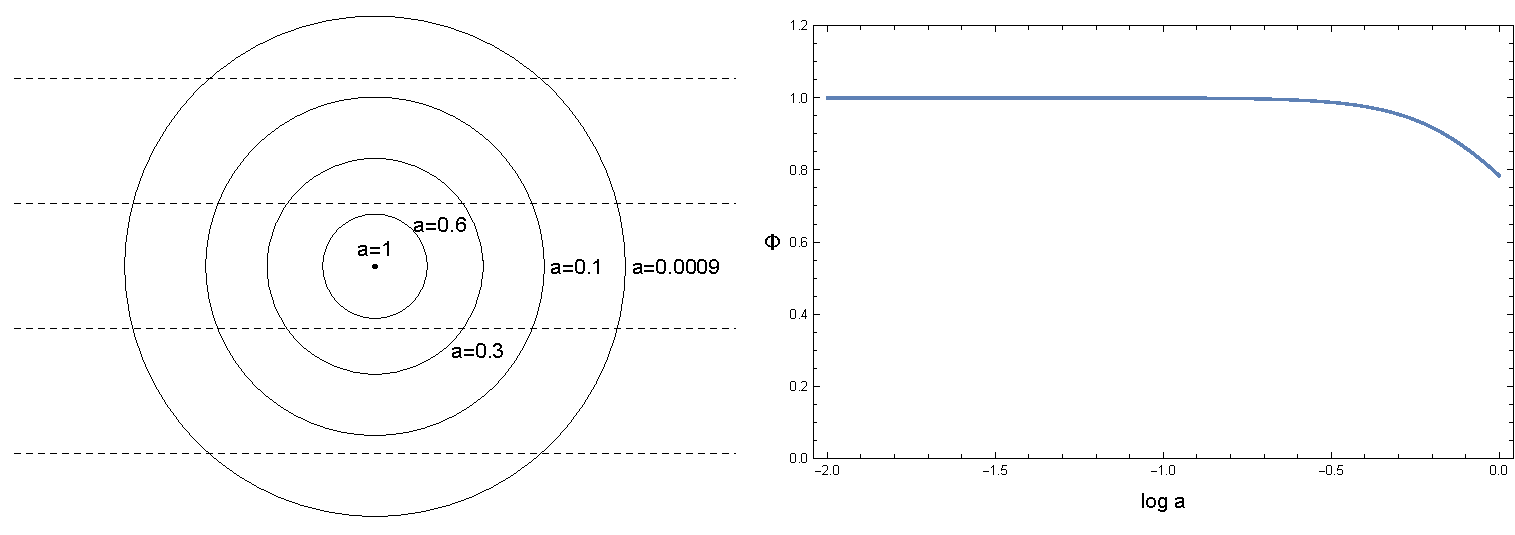
\includegraphics[width=4in]{figures/nsffig1.pdf}
\caption{\small{a) The local Universe interior to the CMB photosphere
expressed in comoving coordinates. The circles are, in order, $a=0.6$,
($z\sim0.7$), schematically the limit of present surveys, $a=0.3$,
($z\sim2$) roughly the effective limit of future surveys, the nominal
Epoch of Reionization at $a=0.1$, ($z\sim9$ and the CMB photosphere at
$a=0.00093$, ($z\sim1100$) and a distance $x_{\rm CMB}\sim13.9$~Gpc. The
comoving radius of the big bang is $14.2$~Gpc. Also shown as dashed
lines are the nodes of a single wave mode with $k\sim0.45$~Gpc$^{-1}$
which contributes significantly to spherical harmonics with $\ell\lo10$.
b) Variation of the amplitude of this wave with scale factor $a$.}}
\end{figure}

\ni{\bf The Inflation of Our Universe:} The flatness of the geometry today, the isotropy of
the CMB temperature, and the very existence of fluctuations with
wavelengths longer than naively allowed by causality are all consistent
with the simplest version of a much more specific and even bolder
conjecture by Guth~\cite{Guth1981}, Linde~\cite{Linde1982a} and others
(e.g.~\cite{Mukhanov:1981xt, Sato1981, Hawking1982, Starobinsky1982,
Albrecht1982, Bardeen1983}), that the Universe underwent a period of
``inflation'' at much earlier times. This theory is based on the idea
that all the structures in the observed Universe emerged from quantum
fluctuations about $10^{-33}$ seconds after the Big Bang. Inflation,
which describes a phase of accelerated cosmic expansion, is the leading
theory providing a causal mechanism for generating these fluctuations
and stretching them to cosmological scales. The microphysics of
inflation makes detailed predictions for the spectra of these
fluctuations as observed in the CMB, in particular a slight tilt in the
power spectrum, which has been measured (see e.g.~\cite{Malik2008,
Gordon2000} and references therein).

%This paragraph is facultative:
Qualitatively, the causal mechanism seeding the primordial perturbations
is easily understood. During inflation, the physical Hubble radius, $H^{-1}$,
which can be thought of as the ``apparent horizon", was roughly
constant. Meanwhile, quantum fluctuations in the matter field(s) and
metric are constantly generated with wavelength $H ^{-1}$ at
most~\cite{BirrellsBook1984}. Once produced, a fluctuation with comoving
wavelength $\lambda$ is stretched with the expansion of space past the
Hubble radius, at which point its dynamical timescale, $\sim ac/k$ was
larger than the expansion time and it ``exited'' the horizon and its
amplitude froze.  Throughout inflation, such fluctuations are
continuously created at the physical scale $H^{-1}$. Therefore, by the
end of inflation, perturbations will finally have been produced on a
whole spectrum of physical scales.


% therory of cosmological perturbations: Lifshitz1946, Lifshitz1963, Bardeen:1980

% --------------------------------------------------------------------

\section{Proposed Research}
\label{sec:research}

The long term goal of this proposal is to connect the CMB to local
surveys by producing an evolving three-dimensional (or in other
words, four-dimensional) map of the Universe that is valid from before 380~kyr to
today, and out beyond 14 Gpc. The exercise is not purely cartographic, as
it is essential that we use secure physical inferences
about the early Universe in making this map. This research was originally envisaged as a three stage program.

The first stage of our proposed program is to use 2D CMB observations alone
to test internal consistency and to recover as much as we can of the 3D
potential, velocity and density fields interior to the last scattering
surface. This stage is nearing completion. In the second stage, we will augment CMB data with existing 3D
measurements from galaxy surveys, gravitational lensing, intermediate
Sachs-Wolfe measurements and so on. This should improve the resolution. This second stage requires detailed and careful analysis of several existing data sets and we request funding to complete the second stage.
% The third stage involves estimating the improvement that should come on
% a decade timescale from future surveys such as LSST and Epoch of
% Reionization investigations, ``Stage IV'' CMB observations, SKA etc.
The third and final stage will be to use our constrained model to make
quantitative predictions about the density field as could be probed
by future surveys, and will include
an investigation of how far it is
possible, even in principle, to reconstruct the structure of the
Universe including what can be inferred beyond our horizon. We anticipate that we will only commence work on this third stage towards the end of the proposed funding but do discuss it here as it is our long range goal.

% - - - - - - - - - - - - - - - - - - - - - - - - - - - - - - - - - -

\subsection{Stage 1. From 2D to 3D: Potential Reconstruction from CMB Data Alone}

During the first phase of our program we are extending our methodology to carry out an independent analysis of the data provided by WMAP and Planck to
investigate of the inflationary paradigm in various different new ways. We
first provide a  brief review of our results so far, to place this
proposed investigation in context.

\ni{\bf CMB Temperature Fluctuation Input Data:}
% Most quantitative cosmology derives from CMB observations.
Observations of the CMB are the foundation on which modern
quantitative cosmology rests. The
conventional way to describe the observations is in terms of spherical
harmonics -- the generalization of Fourier modes to a sphere -- labeled
by $\ell$ and $m$. It is convenient to use an equivalent vector of real
spherical harmonics,
$Y_y(\theta,\phi)=\{Y_{0,0},Y_{1,0},2^{1/2}\Re[Y_{1,1}],2^{1/2}\Im[Y_{1,1}],Y_{2,0},\dots,2^{1/2}\Im[Y_{\ell_{\rm
max},\ell_{\rm max}}]\}$ of length $(\ell_{\rm max}+1)^2$ and where
$\theta,\phi$ are standard spherical polar coordinates. Note that there
are $2\ell+1$ independent, real, basis function in each $\ell$-shell.
Note also that $\int d\Omega Y_yY_{y'}=\delta_{yy'}$. It is convenient
to treat $\ell_{\rm max}$ as a continuous variable by adding a fraction
between zero and unity of the largest $\ell$ shell and therefore
smoothly change the angular resolution. (The use of a real basis helps
identify systematic effects.)

%%%%%%%%%%%%%%%%%%%%%%%%%%%
\begin{figure}[t]
\centering
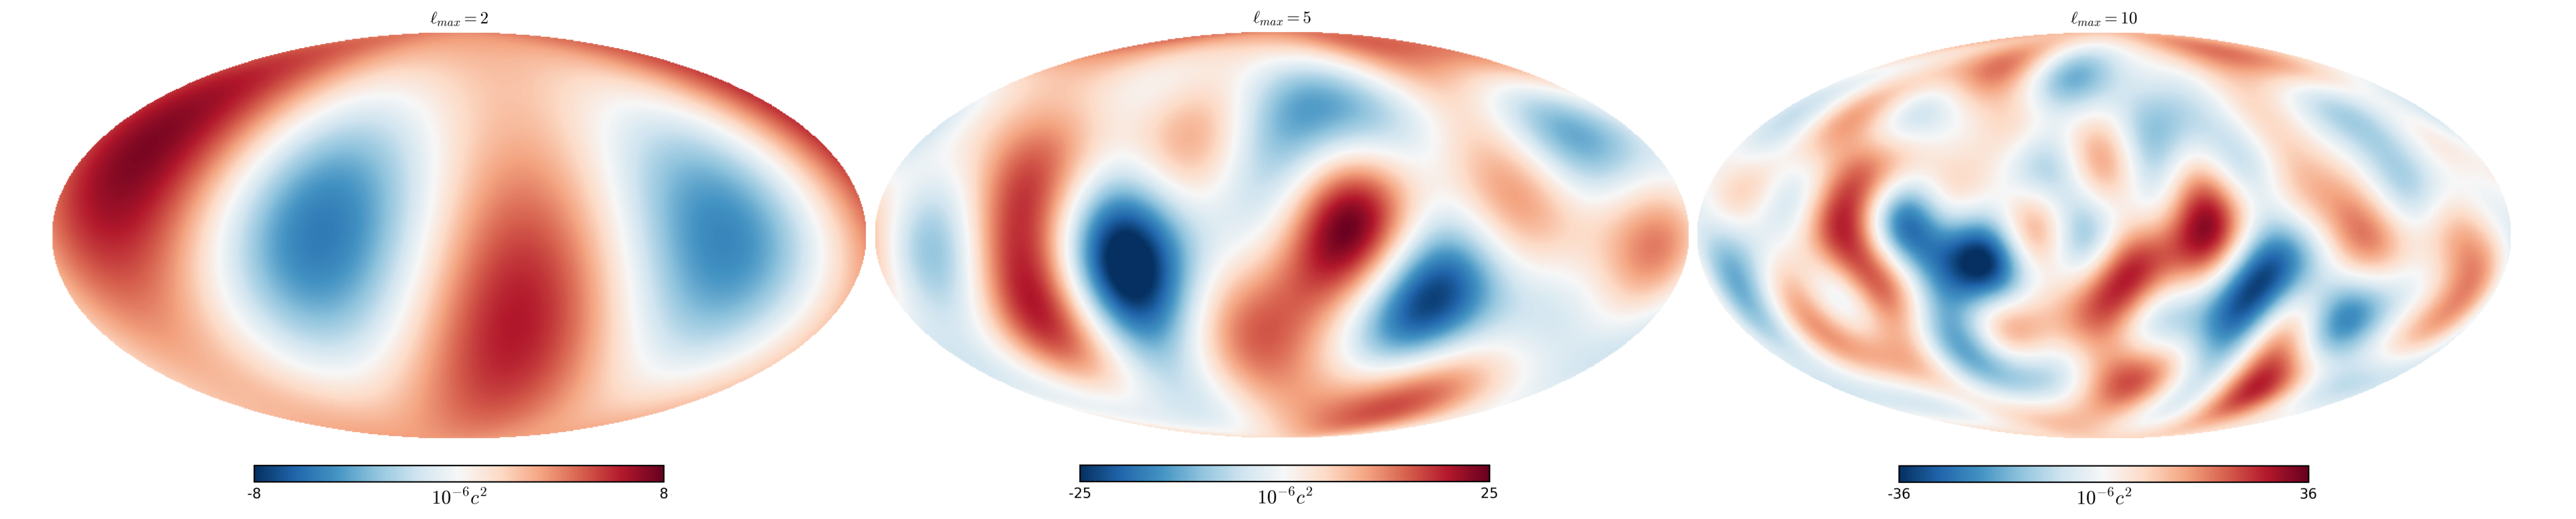
\includegraphics[width=6.5in]{figures/Planck_lmaxs.pdf}
\caption{{\small Photospheric potential fluctuations of the CMB for
$\ell_{\rm max}=2,5,10$ derived from Planck data shown as Mollweide
projections.}}
\label{Fig:placklmaxs}
\end{figure}
%%%%%%%%%%%%%%%%%%%%%%%%%%%

Most investigations have to date focused on measuring the ``power'' in the
temperature fluctuations (including polarization) associated with a
given $\ell$, obtained by summing products of the coefficients of the
harmonic components over $m$, and comparing it with the predictions of
various cosmological models. This program has been wonderfully
productive, and has resulted in the world model outlined in the introduction.
Furthermore this power spectrum has been successfully reconciled with
features of the local Universe, such as galaxy counts. One common
assumption is that the particular realization of the Universe that we
are observing is drawn from a statistical ensemble of universes. When
$\ell$ is large, we have many independent measurements on the associated
angular scale, $\sim\pi/\ell$, and so we can measure an rms value for
the harmonic component with a small variance. However, when $\ell$ is
small, we have only a few such measurements and the ``cosmic'' variance
is large. Despite their great value, these statistical measurements
inevitably discard information which may be valuable.\footnote{This is
in the sense that music is far more than a ``flicker'' power spectrum.
To pursue our musical metaphor, different voices and instruments
contribute different ranges of frequencies to a musical performance over
a total range of roughly ten octaves. We are only listening to the bass
range but higher voices and instruments can still contribute to what we
hear.}  In the proposed study, only one specific realization of the
Universe -- the one we inhabit --  is considered.

In order to start us on a pilot investigation, Planck team members Wehus \&
Eriksen  (Oslo)  kindly supplied us with 100 sample Commander Planck temperature
fluctuation maps for $0\le\ell\le10$ or $1\le y\le121$. From this
ensemble we compute the mean 2D photospheric potential
fluctuation map at the time of recombination, $\Phi=a_yY_y$, up to various $\ell_{max}$ as shown in Figure \ref{Fig:placklmaxs} (including
the monopole and dipole components and adopting the summation
convention) and the covariance matrix $C_{yy'}$ associated with the
harmonic components $a_y$. We find that this matrix is invertible and
can be used directly up to $\ell_{max}=8$. More careful treatment of the data
is needed beyond this. The fractional variance in individual harmonics
varies between $\sim0.0001$ and $\sim0.01$. Undoubtedly, there are
systematic effects present in this data set which need to be explored,
but the accuracy is high enough to proceed without this.
More samples are available on request: we will continue to work with
Wehus \& Eriksen to make sure the data quality keeps up with the
reconstruction methodology as our map resolution increases.

\ni{{\bf Fourier Mode Modeling of the 3D Potential:}
It is convenient to represent the 3D potential $\Phi$ at the epoch
of last scattering
with a Fourier expansion; the
potential at other times is then calculable through simple manipulation
of the resulting
modes. Although the full
spectrum of the Fourier modes we are discussing is continuous in ${\bf
k}$, the fact that our observations are made over a restricted volume
means that we can treat the waves as a discrete Fourier transform of
modes associated with a box in comoving space of side $L$ on which
periodic boundary conditions are imposed. $L$ is chosen here to have a
compromise value of four times the radius of the CMB photosphere,
$13.9$~Gpc which we adopt as our unit of length.
\begin{equation}
\Phi[{\bf x}(r,\theta,\phi)]=\sum_{n=1}^{N/2}[f_n\cos({\bf k}_n\cdot{\bf x})+f_{N+1-n}\sin({\bf k}_n\cdot{\bf x})]
\end{equation}
where the coefficients $f_n$ are also real and
$
 {\bf k}=\Delta k\{n_1,n_2,n_3\}=k\{\sin\theta'\cos\phi',\sin\theta'\sin\phi',\cos\theta'\}$,
  with $n_1,n_2,n_3$ integers and $\Delta k=2\pi/L=\pi/2$.  We restrict the sum to $(n_1^2+n_2^2+n_3^2)^{1/2}\le n_{\rm max}$ and only need consider $\bf k$ over a hemisphere (since the potential must everywhere be real.) We label the coefficients by the index $n$ running from $1$ to $N\sim4\pi n_{\rm max}^3/3$. ($N=6$ through $4168$ for $n_{\rm max}=1$ through $10$.) $\Phi({\bf x})$ can be expanded formally as an infinite sum of Legendre polynomials and approximately as a finite sum:
\begin{equation}
\Phi({\bf x;\ell_{\rm max}})=\sum_{\ell=0} ^{\ell_{\rm max}}(2\ell+1)\sum_{n=1}^{N/2}j_{\ell}(k_nx)P_{\ell}({\hat{\bf k}}_n\cdot{\hat{\bf x}})[\cos(\ell\pi/2)f_n+\sin(\ell\pi/2)f_{N+1-n}].
\end{equation}

\ni{\bf Gaussian Prior:}
Detailed study of the CMB (e.g.~\cite{Aghanim:2015xee, Ade:2015ava}) has
led to the conclusion that the amplitude of each discrete mode with wave
vector $\bf k$ is well modeled as having been drawn from a Gaussian
distribution of variance $\sigma_{\bf
n}^2=\alpha^2(n_1^2+n_2^2+n_3^2)^{-3+(n_s-1)}$, where $n_s$ is the
scalar spectral index. Adopting this model, we can fix the spectral tilt
to the Planck best-fit value (this assumption will be relaxed in the
next subsection in order to estimate the inflationary hyperparameters)
and we fix the reguliarization constant $\alpha$ following the
evidence analysis of~\cite{Suyu2006}. As will be explained below, this constitute the first step towards a hierarchical
modeling of the system where $\alpha$ is one of a set
of hyperparameters governing the statistics of the potential field.


%%%%%%%%%%%%%%%%%%%%%%%%%%%%%%%%%
\begin{figure}[t]
\centering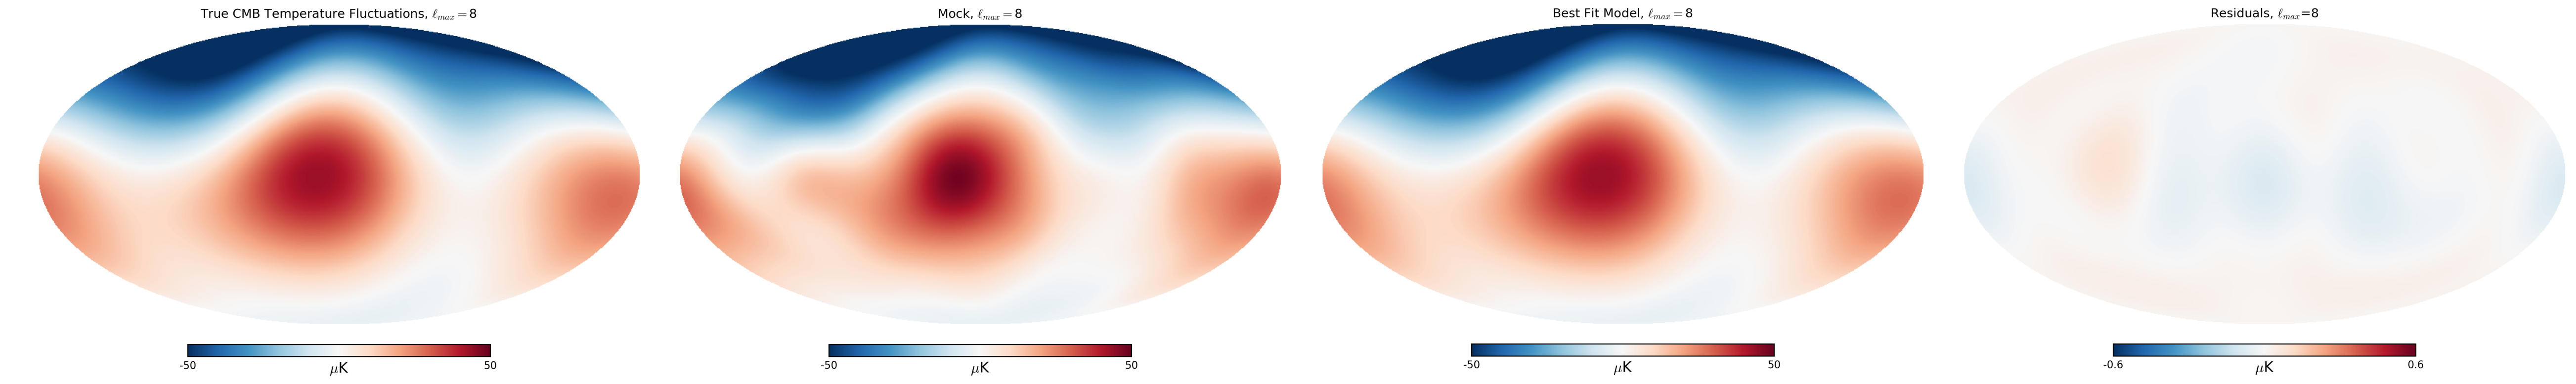
\includegraphics[width=1.\linewidth]{figures/Reconstruction2D.pdf}
\\
\centering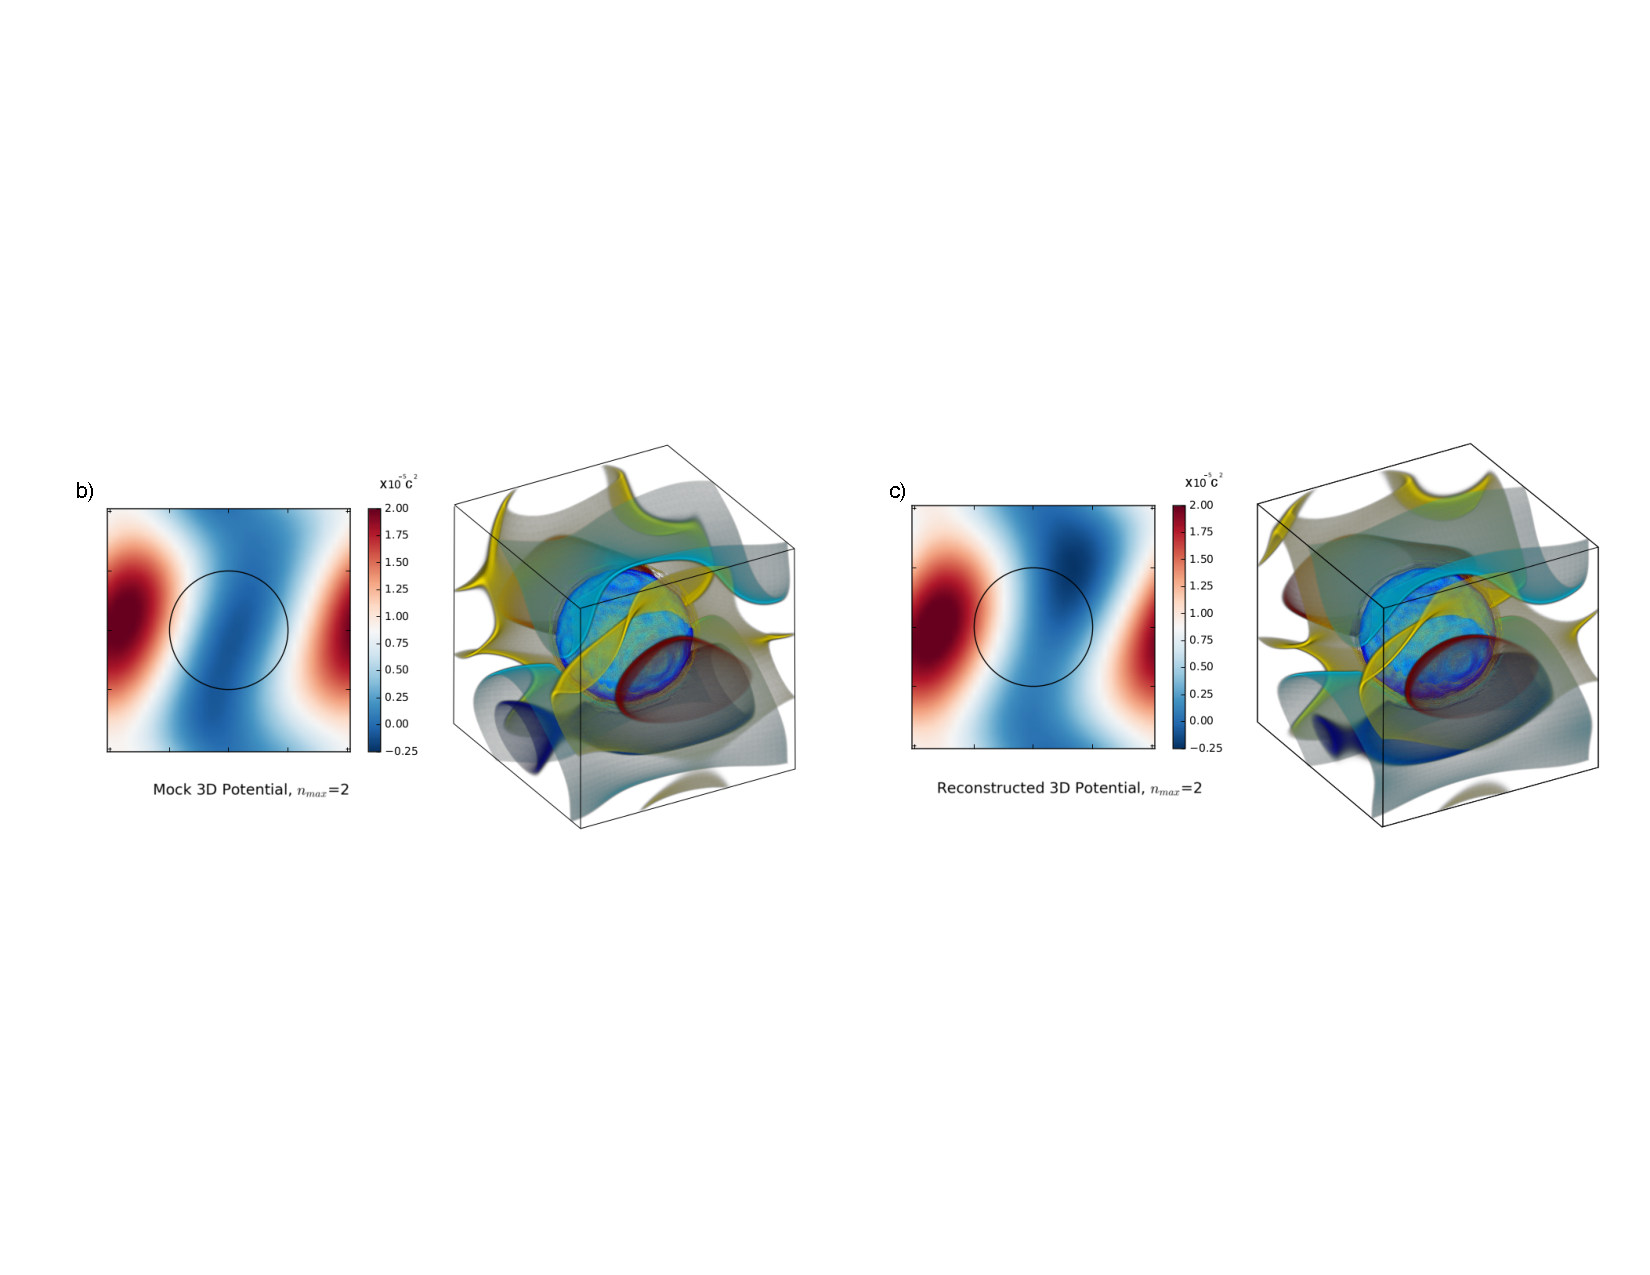
\includegraphics[width=1.\linewidth]{figures/Reconstruction3D-1.pdf}
\caption{{\small
a)  Demonstration of the reconstruction pipeline.  In this pilot study, 81 spherical harmonics and a
Gaussian prior were used to recover 122 Fourier components with
$n_{\rm max}=2$. The monopole and dipole were not removed.
 {\it First panel: } Simulated, noiseless 2D potential fluctuations on the CMB photosphere. {\it Second panel: } Noisy mock observation. {\it Thris panel: } Most probable model, as given by equation \ref{eq:mostprobablemodel}. {\it Fourth panel: } Residuals. As expected, the posterior predicted potential maps have higher uncertainty in the galactic plane.
  b) Simulated 3D gravitational potential at the time
of recombination.  {\it First panel: } Slice of the 3D potential in the
$x_3=0$ plane. The CMB photosphere is represented by the black circle.  {\it Second panel: } 3D visualization of the potential. c) 3D reconstructed potential, recovered from the noisy 2D fluctuations on the CMB photosphere. Both panels a analogous to the ones in b), and show very good agreement between simulation and reconstruction.
}}
\label{Fig:Mockreconstruction}
\end{figure}
%%%%%%%%%%%%%%%%%%%%%%%%%%%%%%%%%


\ni{\bf Preliminary Results:}
The simple question that motivated this investigation, and which did not
seem to have a well-known answer, was how much of the 3D potential could
be reconstructed interior to the 2D CMB photosphere using CMB
observations alone. This is an example of what is sometimes called {\it
holography.} At first sight this might seem hopeless, because if one
associates $\ell_{\rm max}$ with $k\,x_{\rm CMB}$, then we are trying to
solve for $O((k_{\rm max}\,x_{\rm CMB})^3)$ Fourier modes using only
$O(\ell_{max}^2)$ spherical harmonics. However, if we confine our
attention to the longest wavelength waves, and
use all the information that is at our disposal to exploit the high
accuracy of the measurements while accepting uncertainty in the result,
then it is possible to complete this task.\footnote{Our approach is
quite complementary to that of Yadav and Wandelt~\cite{Yadav:2005} who
are concerned with wavelengths comparable with the thickness of the
recombination surface around the acoustic peak near $\ell\sim200$.}


\begin{figure}[t]
\centering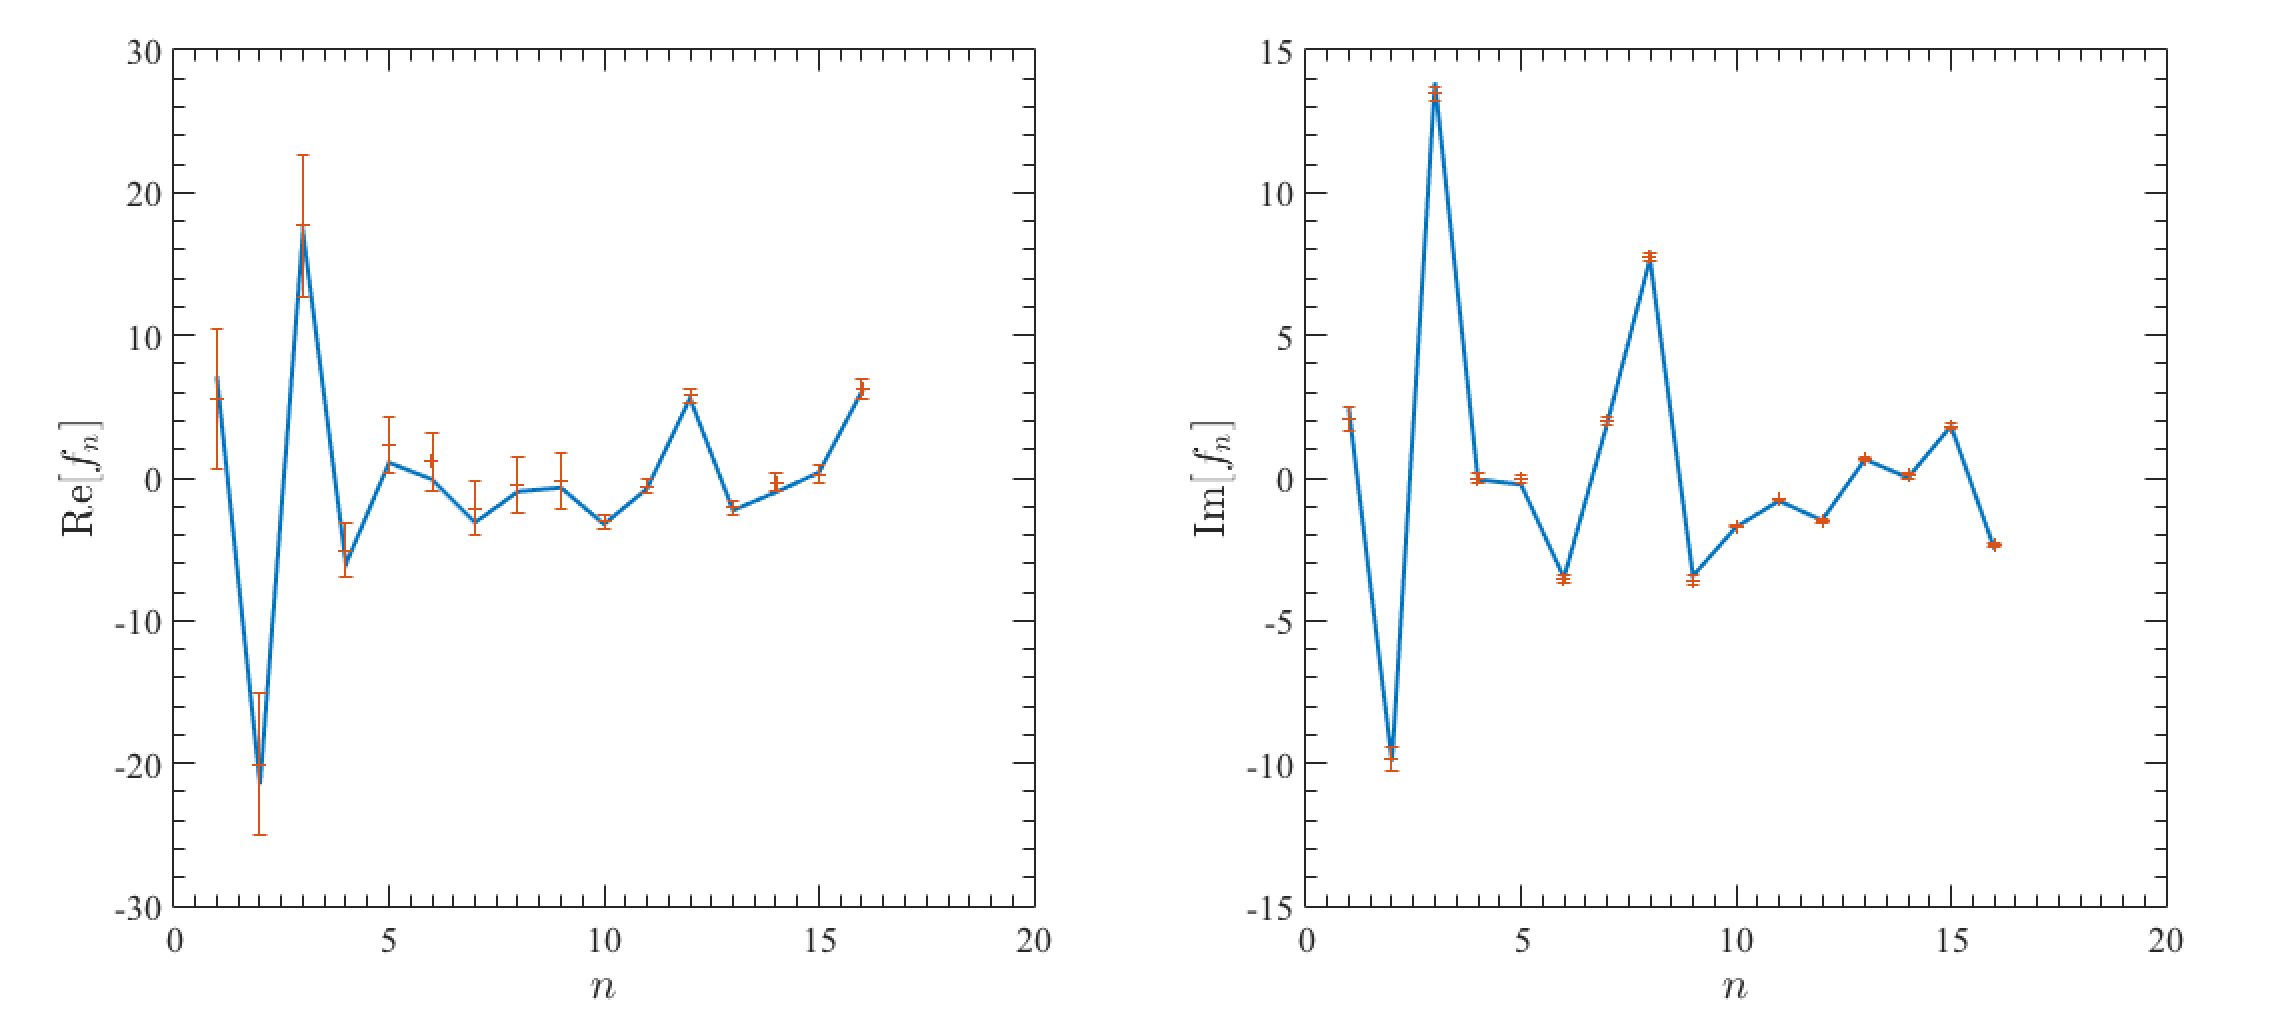
\includegraphics[width=0.7\linewidth]{figures/errorrec.png}
\caption{{\small
Error on the reconstructed $f_n$ parameters in the reconstruction from Figure~\ref{Fig:Mockreconstruction}. The left panel shows the real part of the coefficients while the right panel shows the corresponding imaginary part.
 {\it Blue:} True $f_n$ values. {\it Orange: } Reconstructed $f_n$ values. The error bars are given by the  posterior covariance matrix $\mathbf{A}_{nn'}^{-1}$.
}}
\label{Fig:recerror}
\end{figure}


For a set of $f_n$ parameters, our model for the 2-dimensional sky is defined by computing the spherical harmonic coefficients $a_y
=\mathbf{R}_{yn}f_n$, where the ``response
matrix'' is given by:
\begin{equation}
\mathbf{R}_{yn}=4\pi Y_y(\theta'\phi')j_\ell(k)[\cos(\pi\ell/2),\sin(\pi\ell/2)]\ {\rm for}\ [1\le n\le N/2,\ N/2<n\le N]\, .
\end{equation}

For a given data set of $a_y$ measurements, we approximately characterize the posterior PDF (which under our
assumptions is a multivariate Gaussian distribution) for the
coefficients $f_n$, ${\cal P}\left(f_n|a_y\right)$, by first finding its peak, by minimizing the quantity
\begin{equation}
-2\ln{\cal P}\left(f_n|a_y\right) \approx (a_y- f_n\mathbf{R}_{ny})C_{yy'}^{-1}(a_{y'}-\mathbf{R}_{y'n'}f_{n'})+\frac{f_n^2}{\sigma_{{\bf n}}^2} + \mathrm{const.}
\end{equation}
with respect to variation of $f_n$. Note that $\sigma_{\bf n}$ contains
the normalization $\alpha$.
Here, $C_{yy'}^{-1}$ is the inverse
of the covariance matrix. This leads to the following set of
linear equations, which can be solved using standard library routines:
\begin{equation}
f_n=\left(\mathbf{R}_{ny}C_{yy'}^{-1}\mathbf{R}_{y'n'}+\frac{\delta_{nn'}}{\sigma_{\bf n}^2}\right)^{-1}\mathbf{R}_{n'y}C_{yy'}^{-1}a_{y'}
\label{eq:mostprobablemodel}
\end{equation}

% In Section~\ref{} below, we give a more rigorously-derived expression for the posterior PDF ${\cal P}$.


For the purpose of this pilot study, the modes that mostly concern us remain linear and are ``adiabatic'', so that we need not to worry about secondary effects that usually enter the transfer function. The approximate form given above is sufficient for a feasibility check:
as shown in Figure~\ref{Fig:Mockreconstruction} using mock data, we have found that {\it it is possible to solve for
stable, low order maximum posterior Fourier coefficients, which can
recover harmonic coefficients $a_y$ that are consistent with the
original data.} We have applied this approximate procedure to the
actual Planck data, and our results are exhibited in Figure~\ref{Fig:PlanckRec}.

The error on the recovered Fourier coefficients $f_n$ is given by the covariance of the posterior distribution,
$C_{posterior}=\mathbf{A}_{nn'}^{-1} = \left(\mathbf{R}_{ny'}C^{-1}_{y'y} \mathbf{R}_{yn'}+C_{nn'}^{-1}\right)^{-1}$.
Therefore, the marginalized error on individual reconstructed $f_n$ parameters is given by the square root of the corresponding diagonal elements of $\mathbf{A}_{nn'}^{-1} $. The error on the recovered parameters for the reconstruction displayed in Figure~\ref{Fig:Mockreconstruction} is shown in Figure~\ref{Fig:recerror}



There are
features of the data which we have yet to understand, but this suffices
to illustrate what we hope will be possible. It is proposed to refine
and improve upon this basic approach to obtain the best map we can
based upon the CMB data alone. In particular we intend to set clear,
statistical criteria for assessing when it is significant to add
additional Fourier components to the map. With a better understanding of
the robustness of the inference, we will be equipped to proceed with
our further investigation.
To extend our analysis to larger l, when density and velocity effects are also important. It will become necessary to use the standard transfer function to relate the observed temperature fluctuation to the inflationary perturbations and the contemporary potential (and density) perturbations.

%%%%%%%%%%%%%%%%%%%%%%%%%%%%%%%%%
\begin{figure}[t]
\centering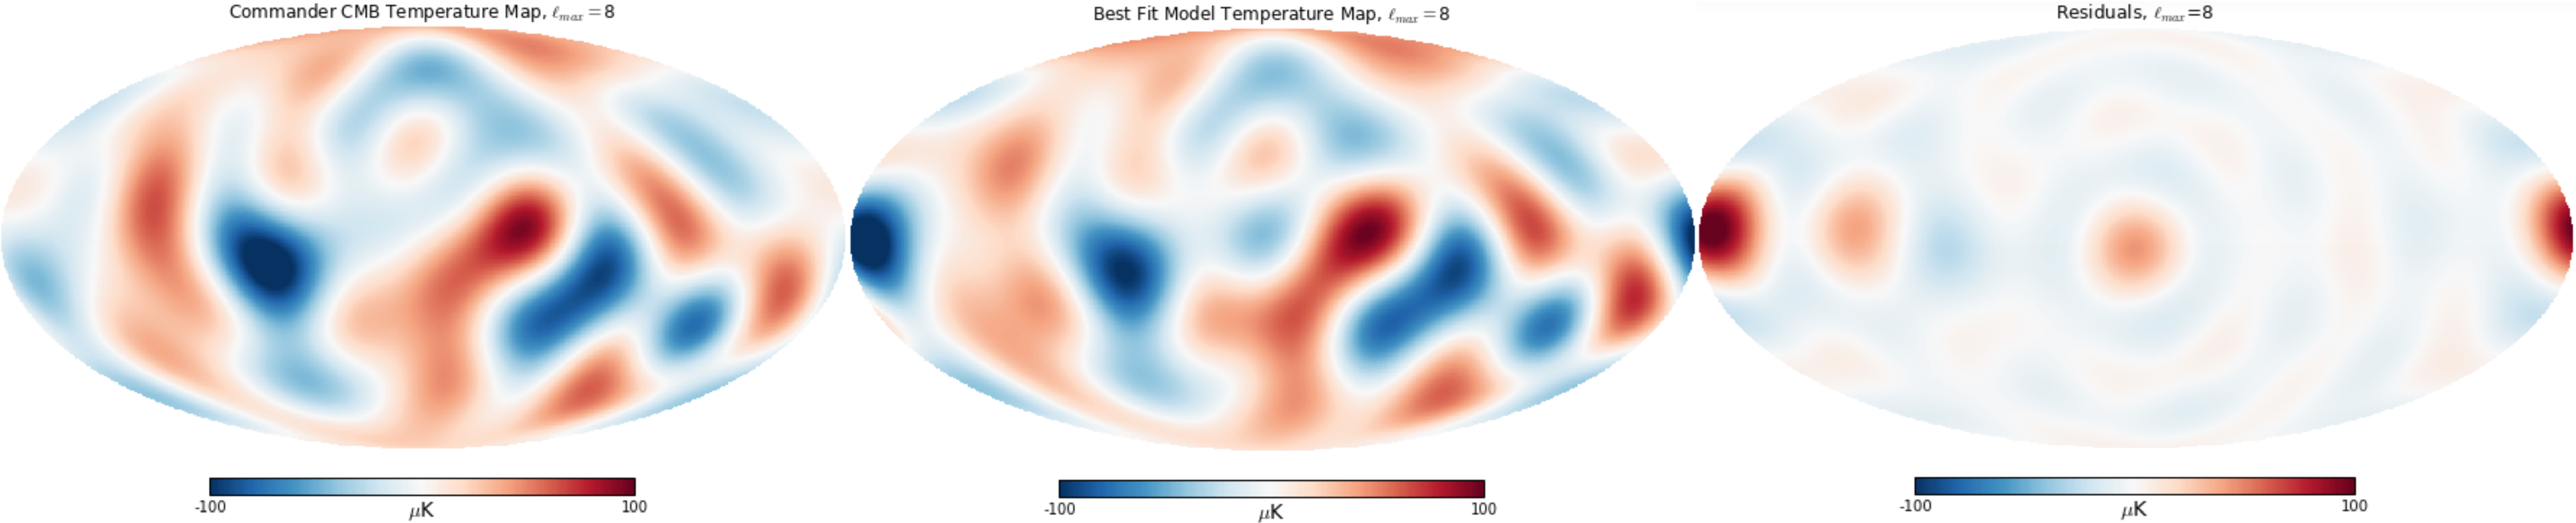
\includegraphics[width=1.\linewidth]{figures/PlanckMoll.pdf}
\\
\centering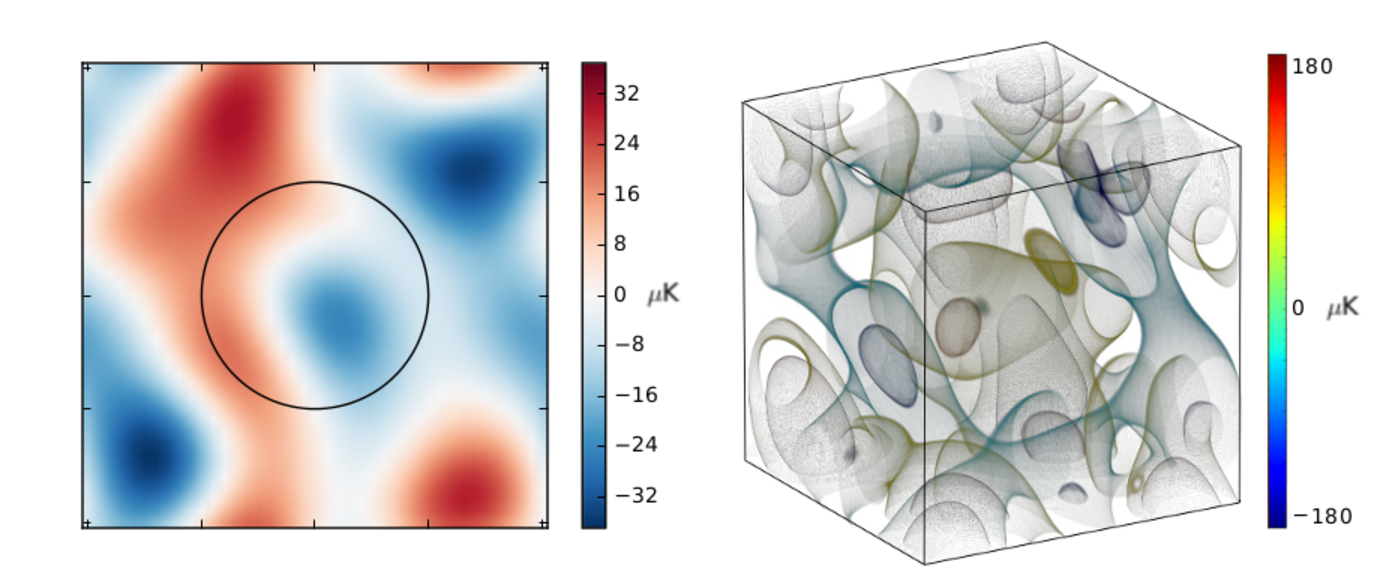
\includegraphics[width=1.\linewidth]{figures/Planck3d.pdf}
\caption{{\small
a)  Reconstruction of the 3D temperature map from the Planck 2D CMB photosphere.  In this pilot study, 81 spherical harmonics and a
Gaussian prior were used to recover 122 Fourier components with
$n_{\rm max}=3$. The monopole and dipole were not removed.
 {\it First panel: } Planck temperature map on the CMB photosphere. {\it Second panel: } Most probable model, as given by equation \ref{eq:mostprobablemodel}. {\it Fourth panel: } Residuals. As expected, the posterior predicted temperature maps have higher uncertainty in the galactic plane.
  b) Slice of the 3D temperature map in the
$x_2=0$ plane. The CMB photosphere is represented by the black circle.  c) 3D visualization of the temperature map. The potential can be obtained by multiplying the temperature map by $1/3$.
}}
\label{Fig:PlanckRec}
\end{figure}
%%%%%%%%%%%%%%%%%%%%%%%%%%%%%%%%%

\ni{\bf Hierarchical Modeling of the Inflationary Origin of Perturbations:}
As explained above, inflation provides a mechanism for seeding
perturbations in the CMB from quantum fluctuations in the early
Universe. The resulting statistical distribution of perturbation
amplitudes provides a conditional PDF for the parameters of the
3D potential in the Universe: {\it inflation provides a physically-motivated
prior for us to use when mapping the potential.} Because we do not know
the exact values of the parameters (or rather, hyper-parameters)
of the inflation model, we must infer them from the data as well, in a
hierarachical model for the CMB data. In this section we step through the
construction of this statistical model.

It is standard, as we shall do here, for most inflation models to assume
that the main matter components during inflation are in the form of
scalar fields.
%, an assumption which shall be adopted in what follows
Moreover, for simplicity, we shall assume that only one scalar field is
dynamically relevant, so that we will work within the framework of
``single-field'' inflation. Apart from these caveats, the framework
developed in what follows will remain model-independent.

We want to describe perturbations of the scalar field, which we call
$\varphi$, about a homogeneous background. It is common to quantify
these perturbations with the gauge-invariant curvature perturbation,
$\zeta$.\footnote{At late times (i.e. after the time of BBN) and inside
of the horizon, when we use the Newtonian gauge to describe the
Newtonian potential $\Phi$, one can think of $\zeta$ and $\Phi$
interchangably. The main advantage of using $\zeta$ during inflation is
that, in single-field inflation, the amplitude of its Fourier modes
remain constant from horizon exit to horizon re-entry, significantly
simplifying their evaluation~\cite{Weinberg2008}.}
%which is defined by:
%\be
%	-\zeta=\psi+H\frac{\delta\rho}{\rho}\, ,
%\ee
%where $\psi$ is the trace part of the spatial scalar metric perturbations, i.e. writing the most general spatial scalar perturbation to a 4-d metric by $\delta g_{ij}=2(\psi\delta_{ij}-E_{ij})$ with $\nabla^2E=0$, then $\psi$ contains the trace of the perturbation. We also define $\rho$ and $\delta \rho$ to be the mean energy density and the linear energy density perturbation, respectively, as well as the $H$, the Hubble parameter.
In the co-moving gauge, the Fourier modes of $\zeta$ as they exit the
horizon are
\be
	\zeta_{{\bf k}}=\sqrt{\frac{\pi}{2}}e^{i\theta}e^{i\frac{\pi}{2}\left(\nu+\frac{1}{2}\right)}(-\tau)^{\nu}\mathcal{H}^{(1)}_\nu(-k\tau)\, .
\ee
Here, $\nu$ is a slowly varying function which encapsulates the specific
dynamics of the inflationary model, $\mathcal{H}^{(1)}_\nu$ is a Hankel
function of the first kind, $\tau$ is the conformal time, defined by
$d\tau=a(t)dt$, and $\theta$ is a random variable endowing each mode
with a random phase. One prediction of inflation is that {\it $\theta$ should
have a uniform probability distribution between 0 and $2\pi$}.

This is a
fundamental prediction of inflation, which stems from the assumption that
the fluctuations are quantum mechanical in origin, the very assumption
the idea of inflation is based upon.
However, the actual distribution of the phases for the modes of $\zeta$
(or $\Phi$) in the CMB has yet to be measured. This is because, so far,
most analyses of CMB data have been restricted to measuring
the power spectrum of
fluctuations, $\Delta_\zeta^2$.
%, defined by
%\be
%	\Delta_\zeta^2=\frac{k^3}{2\pi^2}\mathcal{P}_\zeta \propto |\zeta_{\vec{k}}|^2\,.
%\ee
Because the power spectrum is proportional to $ |\zeta_{{\bf k}}|^2$,
when such a measurement is made, the phase information of the modes is
lost.
Since our proposed hierarchical model explicitly
includes the 3D potential interior to the sphere of last scattering
explicitly,
this phase information will
be readily available:
% Therefore, the new analysis of the CMB data we
% are proposing will make the measurement of the distribution of the
% phases possible.
we will be able to perform a direct test of the quantum
origin of the CMB fluctuations. In Figure~\ref{f:variations} we
show an example visualization of the phases of a mock 3D potential:
a key part of our research program will be to develop
robust statistical
tests of the posterior inferences of such phases, first using realistic
mock data (to avoid {a posteriori} bias),
and then on the Planck temperature map.

\begin{figure*}[t]
\vspace{-1cm}
\begin{center}
\centering
\begin{minipage}[t]{0.48\linewidth}
\centering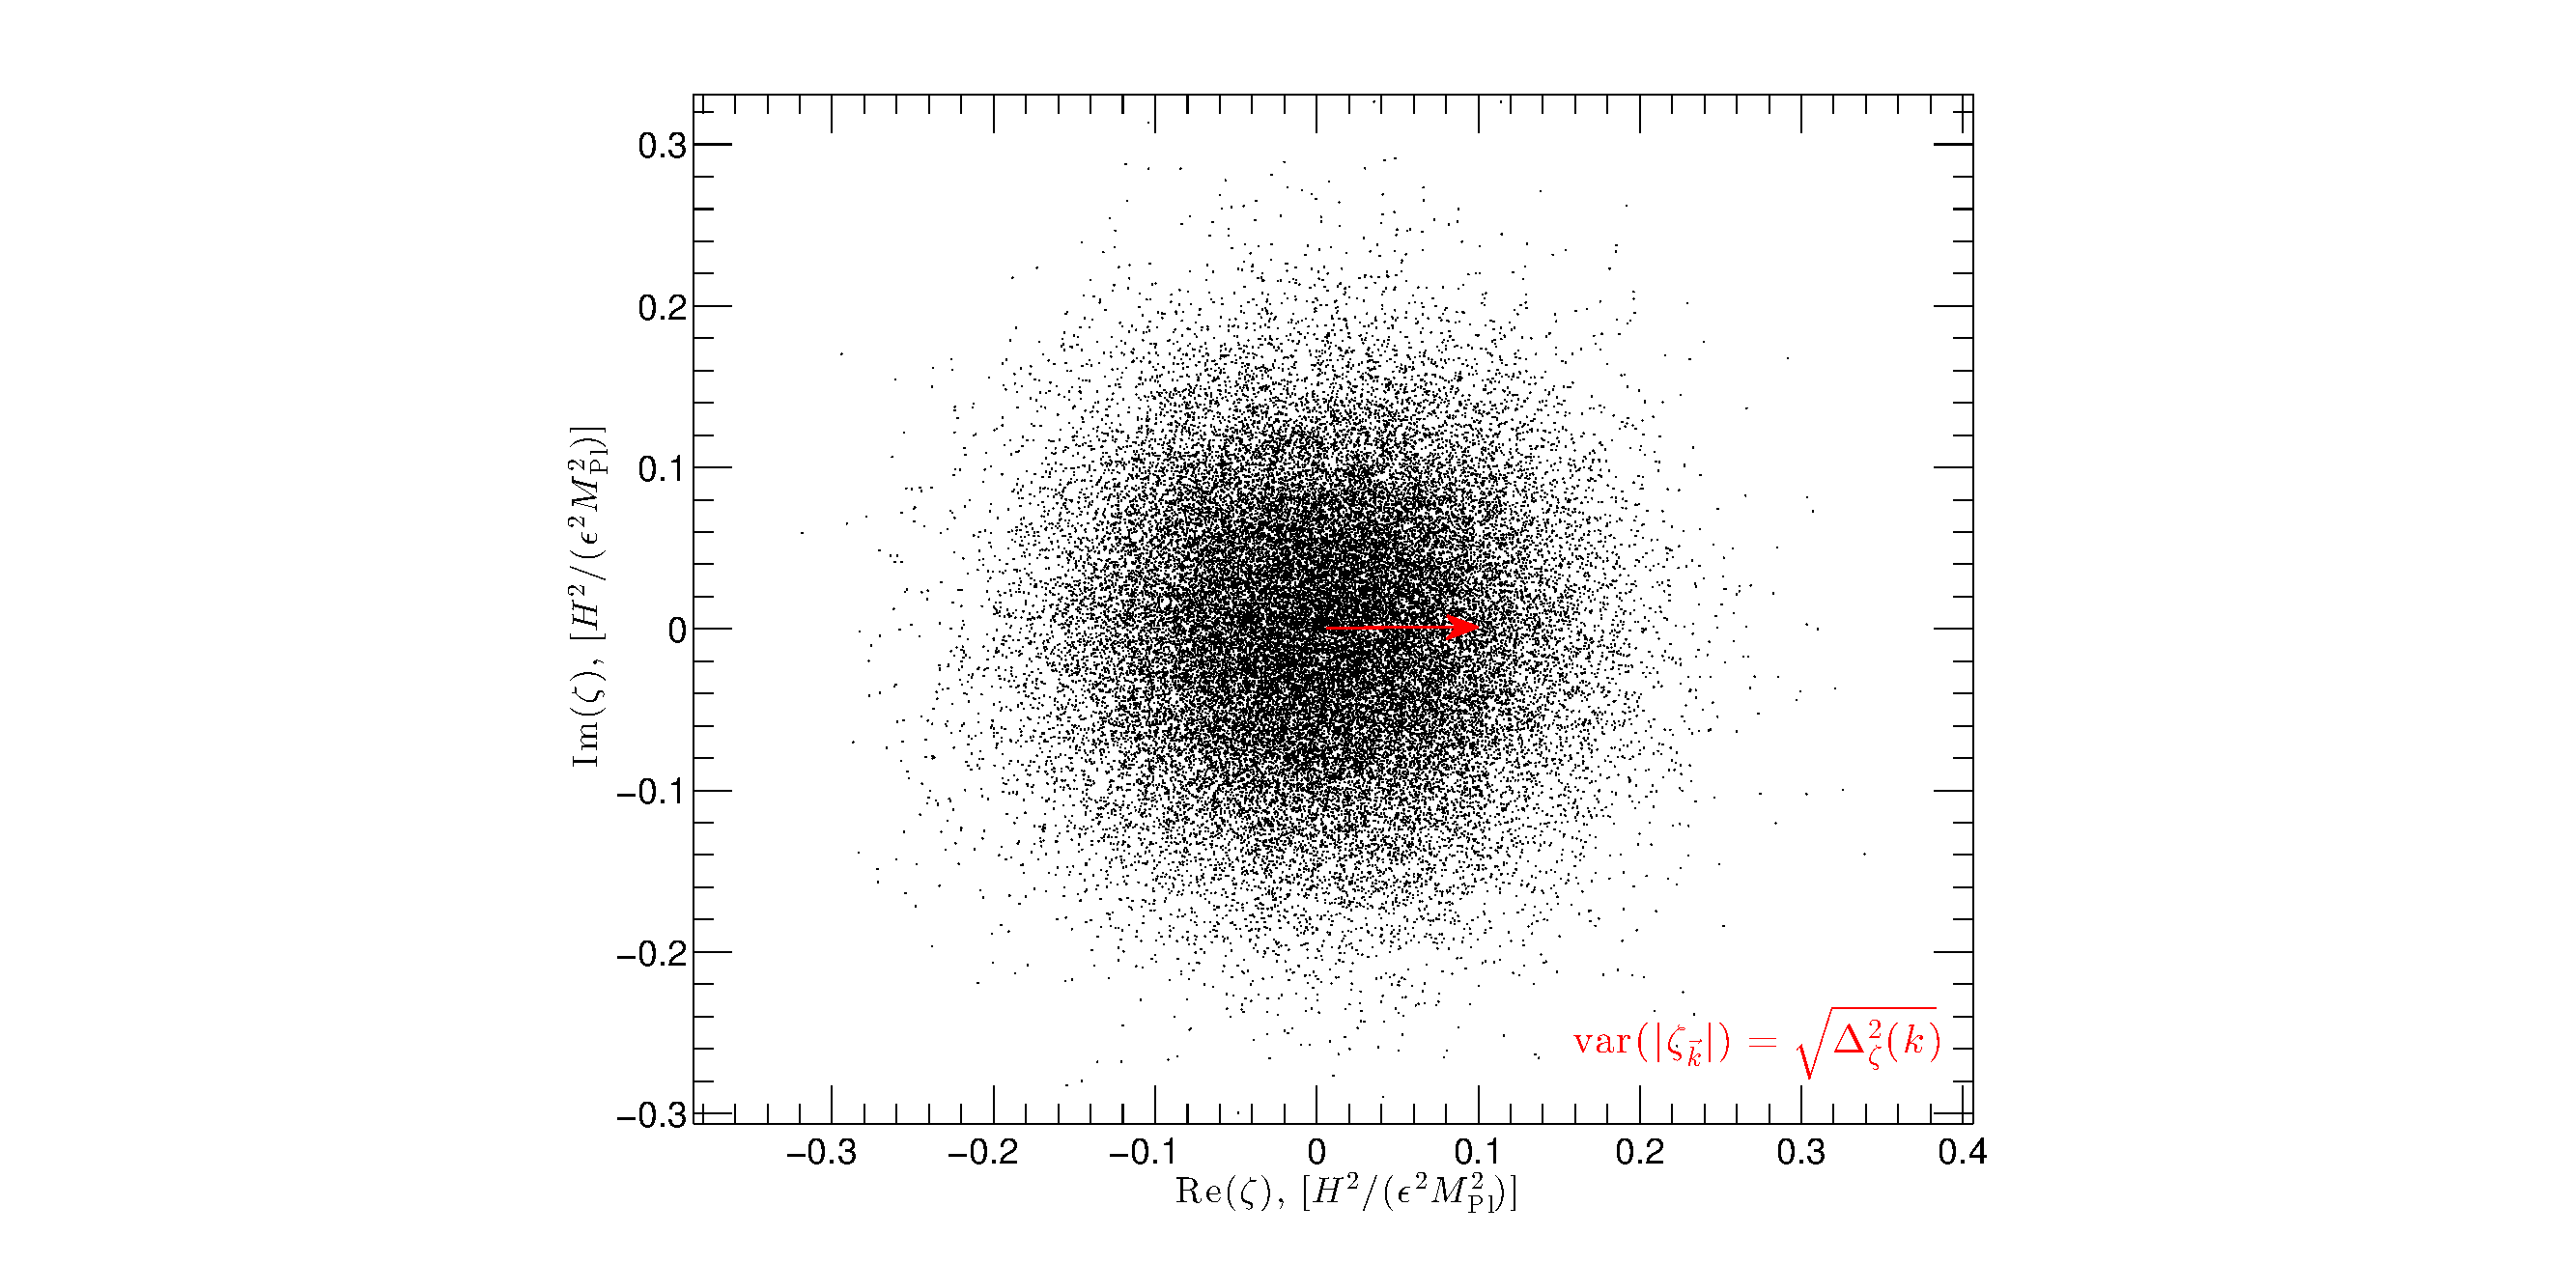
\includegraphics[trim = 80 -32 0 50 mm, width=.8\linewidth]{figures/onemodeThetadist.pdf}\\
\end{minipage}\hfill
\begin{minipage}[t]{0.48\linewidth}
\centering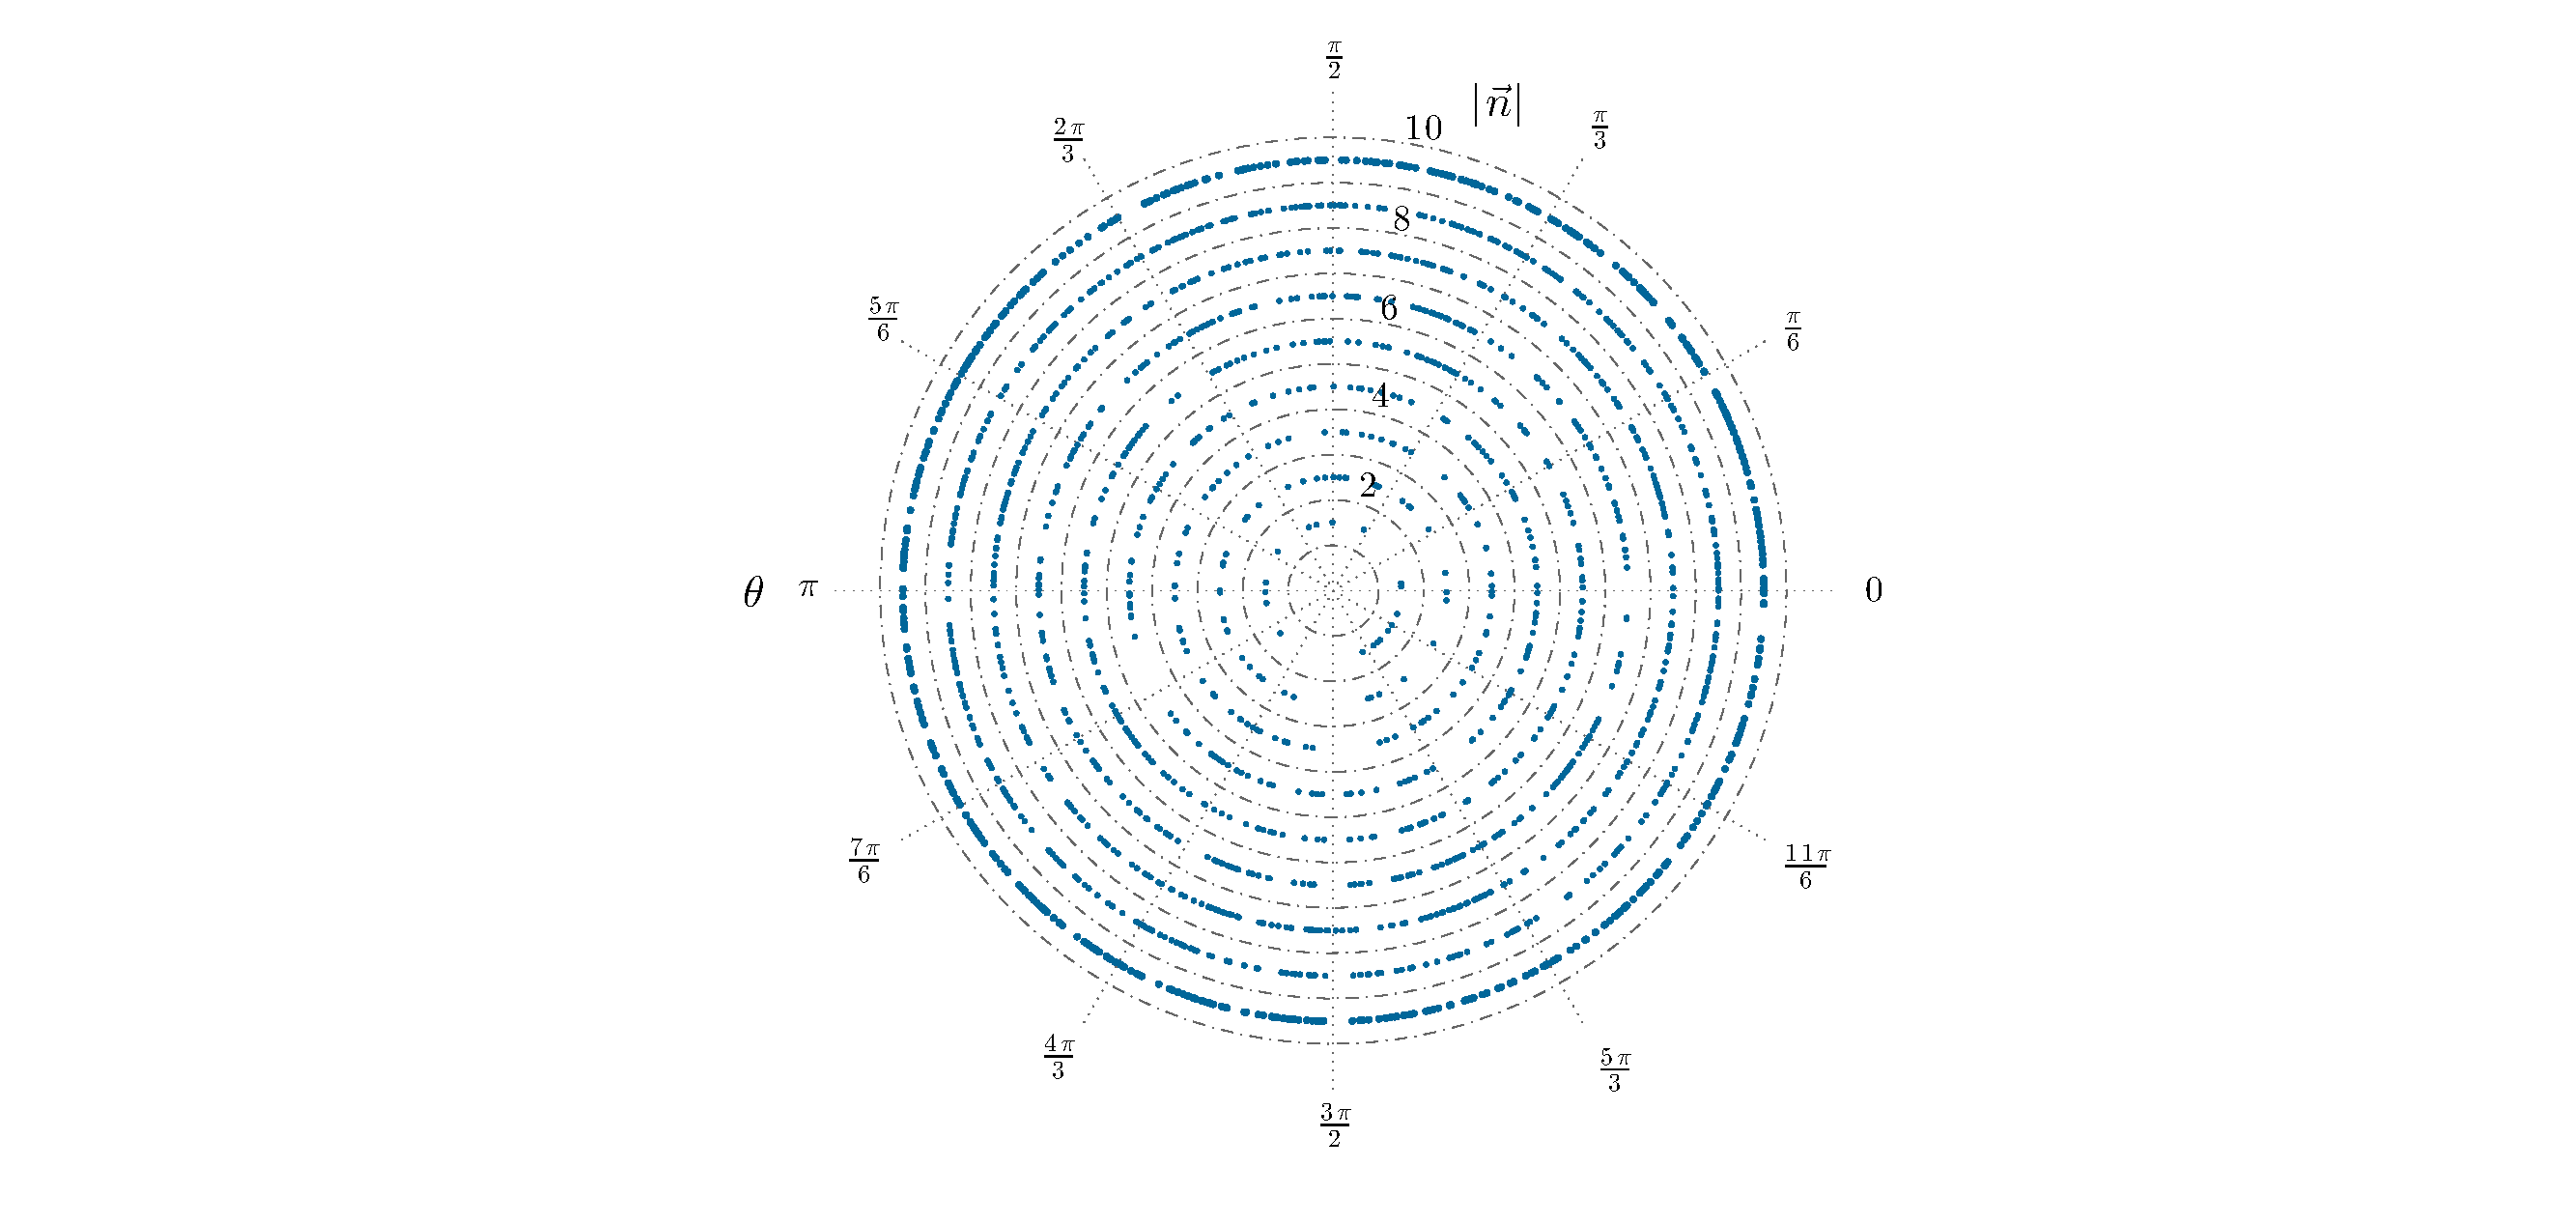
\includegraphics[trim = 0 0 0 0 mm, clip, width=.8\linewidth]{figures/first10modesThetadist.pdf}\\
\end{minipage}
\caption{\label{f:variations}
\small{{\it Left panel}: Distribution of the modes of $\zeta_{{\bf k}}$
at fixed $|{\bf k}|$.} \small{{\it Right panel}: Representation of  the
norm of the first few $k$-modes ($|{\bf n}|$ from 2 to 10), versus their
random spatial angle $\theta$. If the individual modes were clustering
around an angle, this would demonstrate that $\theta$ is actually not a
uniformly distributed random variable, representing a serious challenge
for inflation. Regardless of the distribution of $\theta$, observations
of $\Delta_\zeta^2$ would not be affected. }
\vspace{-1cm}
}
\end{center}
\end{figure*}

One of the main uncertainties pertaining to inflation remains the shape
of the potential for the scalar field $\varphi$, which determines the
specific dynamics of inflation, e.g. its energy scale and the precise
shape of the power spectrum, bi-spectrum, etc. it produces. Using our
low-$k$ 3D reconstruction of the potential $\Phi$, it will  be
possible to {\it reconstruct the inflationary potential over a limited range
of $\varphi$.} This can be achieved by expanding the potential locally around
a fixed $\varphi=\varphi_*$ in
% a model independent way in
terms of the
``slow-roll'' parameters. We can then define the inflationary
hyperparameter vector
\be
	\vec{\eta}=(H^2_*/\epsilon_*,\, \epsilon_*, \,\eta_*, \, (\eta_2)_*, \,(\eta_3)_*)\, ,
\ee
which defines uniquely a shape for the potential around $\varphi_*$.
Here, the star quantities refer to their values when
$\varphi=\varphi_*$.
We then infer the probability
of a given vector $\vec{\eta}$ given the data $a_y$, via the potential
map $f_n$, which we marginalize over,
as
% $\mathcal{P}(\vec{\eta}| a_{y})$,
\be
\mathcal{P}(\vec{\eta}| a_{y})=\frac{1}{(2\pi)^{p/2}} \left[\mathrm{Det}(C_{nn'})\mathrm{Det}(C_{yy'})\mathrm{Det}\,\mathbf{A}_{nn'}\right]^{-1/2}e^{\left\{\frac{1}{2}\mathbf{B}_{n}\mathbf{A}_{nn'}^{-1}\mathbf{B}_{n'}-\frac{1}{2}a^{\mathrm{T}}_{y'}C_{y'y}^{-1}a_{y} \right\}}\frac{\mathcal{P}(\vec{\eta})}{\mathcal{P}(a_{y})}\, ,
\ee
where $\mathcal{P}(\vec{\eta})$ is the prior on the
hyperparameters $\vec{\eta}$,
~$C_{n'n}^{-1}$ is a diagonal matrix with diagonal elements given by
$1/|\zeta_{{\bf k}}|^2$.
Note that this generalizes the simple $1/{\sigma_{\bf n}^2}$ term
in the
Gaussian prior introduced above, by relaxing
the assumption of fixed spectral
index $n_s$ and amplitude $\alpha$.
%\footnote{$C_{n'n}^{-1}$ therefore corresponds to the covariance matrix of the Gaussian prior for fixed $\vec{\eta}$ values}
The $\mathbf{A}$ matrix is defined as above and $\mathbf{B}$ vector are given by:
\be
	\mathbf{A}_{nn'} = \mathbf{R}_{ny'}C^{-1}_{y'y} \mathbf{R}_{yn'}+C_{nn'}^{-1}\, ,\qquad \qquad
	 \mathbf{B}_{n}  = \mathbf{R}_{ny'} C_{y'y}^{-1}  a_{y}\, .
\ee

Generalizing this analytic formalism to include the
inflationary parameters that produce
{\it primordial non-Gaussianities} is straightforward. However, a key
assumption in the implementation of the above inference
is the assumption of a Gaussian prior
for the $f_n$. To exploit the full information present in data samples
containing an increasingly larger range of $\ell$ modes to look
for signs of non-Gaussianity, we will investigate suitable
approximations for a non-Gaussian
$\mathcal{P}(f_n|\vec{\eta})$. These approximations will need to preserve
the computational efficiency of the linear modeling inherent to their
Gaussian precursor; this could be achieved via extensions such as Gaussian
mixture models, or Gaussian processes, depending on the form of the
non-Gaussianity. An alternative route could be to implement
the requisite
non-Gaussian prior directly, and sample the $f_n$ and the $\vec{\eta}$
using MCMC sampling. Hamiltonian Monte Carlo has been shown to
work well in simular situations \cite{JascheAndWandelt2013}; Gibbs
sampling (as used by the Planck team themselves)
could also be a good way to cope with the high dimensionality
of the problem \cite{SeljebotnEtal2014}.

\ni{\bf Detailed Approach Incorporating Planck and WMAP Polarization Data:}
Up to this point, we have only considered the CMB temperature data. We
anticipate making significant gains in map fidelity when we incorporate
the existing polarization data as well. While
these will be more sensitive to systematic effects (such as galactic
dust and synchrotron emission), the additional signal to noise alone
should allow us to make maps of higher spatial resolution. The
prediction of E and B mode CMB polarization at low $\ell$ from a 3D
model potential is more involved compared to the temperature field.
Initial simple Monte Carlo ray tracing experiments suggest that this may
be an instructive way to capture the dependence of the polarized
radiation field on the underlying potential -- a challenge will be to
capture this in a form that preserves our ability to use only the fast
linear inversions described above.

Then, we will carry out an extensive systematic error analysis,
assessing sources of contamination from the various foregrounds (using
the Planck products as templates) and quantifying the robustness of our
results to them. We expect all our inferences to increase in precision
as a result of including the polarization information; whether we can
reach the commensurate degree of accuracy will depend on both the
computational and modeling problems outlined here.


% NOTE: they say this in the guidelines:
%
% In addition, proposals may not anticipate future public data releases.
% The scientific case for any proposed investigation must be based on -
% and executable with - data that are in the public domain at the time of
% the original proposal. Any proposal that invokes the use of data that
% are not public at the time of the ADAP 2016 proposal submission deadline
% (other than that explicitly allowed under Section 1.3.4) will be ruled
% noncompliant and will not be rated or considered for funding.

\ni{\bf Tree Representation and Non-Parametric Investigation of Gaussianity:}
There is another way to think about this problem. Let us build up the
resolution of the potential on the CMB photosphere by increasing $\ell$
continuously from zero. Saddle points -- designated  S -- accompanied by
extrema -- either maxima, designated H,  or minima, designated, L --
will be created. They will be accompanied by fresh separatrices -- the
contours that pass through the saddles. These come in two types -
``lemniscates'', like an infinity symbol, and designated X, and ``lima\c
cons'', with the shape of a pinched annulus, and designated
K~\cite{Blandford:1986}. New separatrices may be created between
existing separatrices or out of a contour encircling a $L$ or a $H$.
Occasionally, the inverse process -- annihilation -- will occur. If we
designate the total number of maxima, minima, saddles, lemniscates and
lima\c cons by $N_H,N_L,N_S,N_X,N_K$, respectively, then clearly
$N_S=N_X+N_K=N_H+N_L-2$.\footnote{It is also instructive to calculate
the Hessian matrix for the potential on the sphere and divide the sphere
into ``H-zones'' (where both eigenvalues are negative), ``L-zones''
(where they are both positive) and ``S-zones'' (where they have opposite
signs). These ``curvature maps''~\cite{Nye:1978} are complementary to
the tree representation.}

The nesting of these contours defines a specific topology which suffices
to describe all the equipotentials. It is convenient to represent it
using a ``tree'' containing ``forks'' (corresponding to separatrices and
labeled K or S ), and branches terminating on ``leaves'' (corresponding
to extrema and labeled H or L)~\cite{west2001introduction}. There is
only one ``path'' connecting any two leaves. Although our investigation
has only begun, it is already clear that the statistics and structure of
the tree, satisfy many rules if the underlying fluctuations are truly
drawn from a random distribution, for example $N_K\sim N_X$ as
$\ell\rightarrow\infty$. We propose to explore this novel approach to
testing Gaussianity. We can actually extend this 2D approach on the
photosphere to a 3D approach\footnote{Another generalization that we
plan to explore is describe the topological arrangement of the
polarization patterns~\cite{Scheuer:1977}.} exploring the nesting of the
equipotential surfaces within the photosphere. This leads to similar
type of tree. Although these trees are essentially topological, they can only be measured in 3D if there is very careful control of the systematics in the data.
\begin{figure}[t]
\centering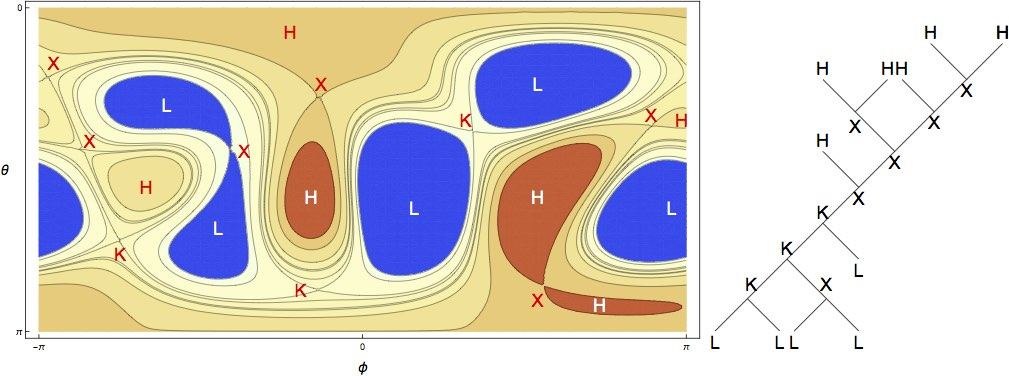
\includegraphics[width=0.6\linewidth]{figures/nsffig5.jpg}
\caption{{\small a) Nesting of separatrices for Planck data, with
$\ell_{\rm max}=4.5$. The extrema, H, L and saddles, K, X are
identified. b) Equivalent tree describing the same data.}}
\end{figure}


% - - - - - - - - - - - - - - - - - - - - - - - - - - - - - - - - - -

\subsection{Stage 2. From 3D to 4D: Incorporating Existing ``Local'' Volumetric Data}
% Producing Maps at Higher Resolution}

At the end of Stage 1, we will have in hand the posterior PDF for the
Fourier mode amplitudes of a 3D model of the potential on large scales
throughout the observable Universe (and slightly beyond) at the epoch of
last scattering.
Our main goal in Stage 2 which is the principal object of this proposal
is to improve the linear resolution of our map as far as we can.
If we now assume a  Friedman-Robertson-Walker expansion
model, with suitably-parameterized expansion rate and a particular
choice of those expansion parameters,  we can evolve the Fourier modes
of any sample potential map we draw  from this PDF forward in cosmic
time in order to make posterior  predictions about the local
$z << 1000$ Universe. The likelihood of these predictions given various
observations in the local Universe will allow us to downweight some
possible models, and hence further reduce the uncertainty in the map.
As we discuss below, the process of combining CMB data with local surveys
will not always be as straightforward as this simple picture of
prediction and evaluation: Stage 2 of this program will involve
investigation of how to carry out the joint inferences robustly and
efficiently.

\ni{\bf CMB Lensing and ISW Measurements:}
An important way to add 3D information on the potential throughout a
significant fraction of the Universe's volume is to include the lensing
of the CMB~\cite{Planck2015cosmopara}. A uniform CMB is unchanged by
gravitational lensing. However, if there is a gradient in the background
temperature, intervening structure will appear as extra power on the
scale of intervening large scale structure.\footnote{More subtle
manifestations including those involving polarization are
possible~\cite{Hu:2002}, but this is the main effect.} The consequences
are largest on much smaller scales than those in which we are primarily
interested. However there are still integral effects with
$\ell\sim30-100$ which are relevant. Furthermore the intense interest in
the claim that inflationary B-modes have been
detected~\cite{Planck2015cosmopara}  has focused much observational and
analytical effort on this region of the spectrum. It is proposed to see
if the addition of these measurements will improve the specification of
the 3D body modes.

Note that in the case of CMB lensing, it is the same 3D potential model
that will be predicting both the lensing effect on the CMB temperature
map (due to structures at $z < 1000$), and  also the intrinsic structure
in this ``background'' temperature map (at $z \sim 1000$) itself. The
consequence will be a non-linear system, which will need to be treated
with care in the inference. The posterior PDF for the Fourier modes will
no longer have a Gaussian form, but the weakness of the lensing effect
may leave it to be close enough to Gaussian for a simple Gaussian
approximation to give sufficient accuracy. This will be the starting
point for our research in this area, which may develop into an
exploration  of better approximations to the posterior PDF for the
Fourier modes  which retain as much of the the computational efficiency
as the linear model as possible.

Similar remarks apply to the Integrated Sachs Wolfe effect which is
caused by variation in the potential over time, attributable to the
cosmological constant (or a ``dark energy'' component) at late times.
It is proposed to see if such
measurements can also contribute to the specification of structure on
the largest scales.
% although here the challenge seems even greater.

\ni{\bf Galaxy Surveys and the ``Local'' Universe:}
Most of the use of galaxy surveys to date has been for drawing statistical inferences
relating the growth of structure to the CMB emphasizing shorter length
scales, notably those associated with BAO and the largest voids
$\sim0.1$~Gpc. However, these same surveys can also be used to augment
the long wavelength CMB data and improve the accuracy and resolution of
the resulting 3D potential map. A good example is the
he all-sky survey made by the WISE satellite.\footnote{https://www.nasa.gov/mission\_pages/WISE/mission/index.html}
Another example is the SDSS/BOSS
program,\footnote{http://www.sdss.org} which covered nearly a third of
the sky with over a million redshifts and photometry on galaxies out to
$z\sim0.7$.\footnote{21 cm redshift surveys provide an important
complement to optical surveys but the survey volumes to date are
comparatively modest.} For our purposes this translates to a comoving
volume $\sim50{\rm Gpc}^3$, about 0.005 of the total. Surveys of much
rarer quasars and the brightest star forming galaxies which extend to
$z\sim6$ provide much greater volumes over which the potential on Gpc
scales can be estimated, albeit with inferior precision.

It is helpful at this point to consider a volume limited-survey of
objects out to some radius~$r$. Suppose we have a set of objects,
($L^\ast$ galaxies, quasars, bright, star-forming galaxies $\dots$) with
space density~$n$, and we want to measure the amplitude of a given
Fourier component with wave vector~$k$ of the relative density
perturbation associated with this potential
$\delta\sim-2k^2\Phi/3a^2H^2$. Now, the accuracy with which the amplitude
of a single relative density perturbation Fourier mode can be measured
is comparable to the precision with which the fractional density
perturbation can be measured in a single region of size equal to the
associated length scale. This is $\sim k^{3/2}n^{-1/2}$, and must exceed
$\delta$. This suggests that the density of such objects must exceed
$\sim H_0^4/c^2\Phi k_{\rm max}$,
and systematic effects must be adequately controlled in order to connect
local surveys with the CMB. We propose to carry out a careful study
based upon trial data to determine when this  is possible.
If this is achievable
using currently available data, as our exploration so far suggests is the case,
then although the data increment will be small, its value
will be much greater because it can act as a {\it phase reference} for
anchoring the imperfectly specified modes measured by CMB observations.

One possible starting point for this part of the program could be to
focus on existing weak lensing surveys, such as in the 1.5 square degree
{\it HST} COSMOS field \cite{MasseyEtal2007}, supplemented by the
publically-available 150 square degree {\it CFHTLens} dataset
\cite{HeymansEtal2012}. These datasets could provide
low signal to noise measurements of the long wavelength potential
fluctuations along the line of sight to about $z \approx 1$,
through  a quantitative comparison with our model predictions.

% - - - - - - - - - - - - - - - - - - - - - - - - - - - - - - - - - -
%
% \subsection{Stage 3. Future Surveys}
% Many facilities that are being planned or built will provide data
% relevant to our approach. In this phase of our program we will use
% simulated data for a selection of these future surveys to make forecasts
% of how our maps should improve, and look for new opportunities to
% exploit them.
%
% \ni{\bf Ground-based CMB Telescopes:}
% While there are exciting proposals for future space-based CMB
% measurements, most attention is currently focused on the next two
% generations -- Stages 3 and 4 -- of ground-based CMB telescopes, which
% have been proposed to deliver results in very roughly five and ten years
% respectively. While these are mostly focused on probing the physics of
% inflation and cosmological neutrinos
% \cite{CMBS4Inflation,CMBS4Neutrinos}, they will also improve the
% measurement of CMB temperature and E-mode polarization on the scales
% $\ell\lo200$ in which we are primarily interested, with signal to noise
% $\sim3\times10^{-4}$, roughly ten times higher than Planck.

% \ni{\bf Survey Telescopes:}
% Construction has begun on the Large Synoptic Survey Telescope
% (LSST\footnote{http://www.lsst.org/lsst/}), which will commence a
% decade-long survey in 2022. It will survey half the sky from Chile (with
% consequently very strong overlap with the ground-based CMB observations)
% in six optical and near infrared bands, detecting about ten billion
% galaxies out to $z\sim2$ for $L^\ast$ galaxies and $z\sim6$ for bright,
% star-forming galaxies and quasars \cite{LSSTOverviewPaper}. Its primary
% cosmological goal is to perform a multi-probe joint analysis (involving
% weak lensing, galaxy clustering, type Ia supernovae, time delay lenses
% and cluster number counts) to see if dark energy (and not just a
% cosmological constant) is responsible for cosmic acceleration
% \cite{LSSTDESCWhitePaper}. However, it  will, in practise, contribute to
% many more important cosmological tests. LSST will only provide
% photometric redshifts, but these will be well-calibrated by large
% spectroscopic surveys including that of
% DESI\footnote{http://desi.lbl.gov}, which is projected to measure
% $\sim20$ million redshifts to $z\sim1$ starting in 2018, and,
% potentially, the all-sky SphereX
% mission.\footnote{http://spherex.caltech.edu/} A complementary source of
% new local data will be the Euclid space
% mission\footnote{http://www.euclid-ec.org}, which is scheduled for a
% 2020 launch and which will carry out weak lensing, baryon acoustic
% oscillation and redshift space distortion measurements using 1.5 billion
% galaxies and 50 million redshifts over more than a third of the sky
% \cite{EuclidSciBook}. The proposed WFIRST-AFTA
% {http://wfirst.gsfc.nasa.gov} also has an impressive program in
% observational cosmology \cite{WFIRSTReport2015}, that will build on the
% LSST and Euclid surveys \cite{JainEtal2015}. Meanwhile, at radio
% wavelengths, the Canadian High Intensity Mapping Experiment
% (CHIME\footnote{http://chime.phas.ubc.ca}, see e.g.\ \cite{CHIME}) will
% measure BAO out to $z\sim2.5$ over half the sky.
%
% As with the CMB, weak lensing and galaxy clustering observations can
% provide ``tomographic'' distance information and, in principle, should
% lead to a better map of the long wavelength potential perturbations.
% Systematic error control on these large scales is as yet uncharted
% territory: our 4D potential maps may have a role to play in this,
% effectively regularizing the local analysis on the largest angular
% scales. At the same time, local constraints on the 3D potential will pin
% down the  model considerably, improving our constraints on the inflation
% model.
%
% \ni{\bf Epoch of Reionization:}
% There is a large effort underway to probe the Epoch of Reionization,
% (EoR) $6\lo z\lo30$ through hydrogen line measurements. This is an
% exciting area of discovery, as the relevant physics depends upon many
% factors, notably first star formation and galaxy assembly that are very
% hard to anticipate.\footnote{JWST (http://www.jwst.nasa.gov), scheduled
% for launch in 2018, will also help indirectly in understanding the
% Universe during this epoch but seems unlikely to provide quantitative
% measurements of very large scale structure.} The experiments will probe
% an ideal range of comoving radius $\sim8-12$~Gpc, interpolating between
% the CMB photosphere and local surveys,  for either contributing to or
% expanding upon our incorporating our 3D potential map.
%
% On a longer time scale there are ambitious plans to construct an
% international Square Kilometer Array
% (SKA\footnote{https://www.skatelescope.org}). The long term goals
% include measuring the redshifts of a billion galaxies, performing weak
% lensing surveys and carrying out more sensitive surveys of the epoch of
% reionization (see  \cite{SKACosmology} and references therein). It is
% likely that the SKA capabilities and schedule will become better-defined
% over the lifetime of this proposed research program.
%
% With a 4D potential model constrained both at $z=1100$ by the CMB and at
% $z=0.5$ by the Dark Energy surveys of the previous subsection, we will
% be able to make predictions about the large scale structure present in
% the volume at $6\lo z\lo30$ probed by EoR surveys. Such a prediction
% should assist in the interpretation of the survey data, and increase the
% fidelity of the measurements made there.

% - - - - - - - - - - - - - - - - - - - - - - - - - - - - - - - - - -

\subsection{Stage 3. Posterior Predictions and Ultimate Limits}
\label{sec:research:stagethree}

The final stage of our research program,
which is likely to be prosecuted towards the end of this proposal period,
will be predictive in
character. A fully constrained 4D model of the large scale gravitational
potential in the Universe, with well characterized posterior PDF, will
enable us to make predictions, with uncertainties, about the  density
field probed by a number of different upcoming sky surveys
and proposed space CMB missions, such as LiteBIRD and PIXIE. Beyond the
fundamental scientific importance of making, and so enabling the testing
of, such predictions, our map will provide a new tool for the
teams analyzing these future surveys. Systematic error control on these
large scales is as yet uncharted territory: our 4D potential maps will
enable the effective regularization of the analysis of
new data on the largest angular scales, and thus potentially provide a
higher contrast view of any anomalies present.

Over the next decade, a suite of all-sky (or at least, wide field)
cosmological galaxy surveys are planned, including those to be carried
out with
LSST\footnote{http://www.lsst.org/lsst/}),
DESI\footnote{http://desi.lbl.gov},
SphereX\footnote{http://spherex.caltech.edu/},
Euclid\footnote{http://www.euclid-ec.org},
WFIRST-AFTA\footnote{http://wfirst.gsfc.nasa.gov}, and
CHIME\footnote{http://chime.phas.ubc.ca}.
We will be able to make predictions about the large scale density
of galaxies and clusters of galaxies, as well as the large scale
tomographic weak lensing density fluctuations, that will be probed by
these surveys.

There is a large effort underway to probe the Epoch of Reionization,
(EoR) $6\lo z\lo30$ through hydrogen line measurements, with facilities
such as the planned Square Kilometer
Array\footnote{https://www.skatelescope.org} and its precursors. This is
an exciting area of discovery, as the relevant physics depends upon many
factors, notably the formation of the first stars and galaxies,  that
are very hard to anticipate. We will be able to make predictions about
the large scale structure present in the volume at $6\lo z\lo30$ probed
by these surveys. Again, such a prediction should assist in the
interpretation of the survey data, and increase the fidelity of the new
measurements made there.

It is also of interest to consider the limitations to what could be
learned in principle about the idiosyncratic structure of our Universe
with {\it any} conceivable observing facility. The many galaxy and EoR
surveys referred to above, combined with CMB lensing and ISW
measurement, should ultimately be able to give a quite detailed
description of 4D potential. Exactly how detailed the map can be made
is an interesting question to ask, and in doing so anticipate being led
to new applications of our approach.
% though the resolution during the dark ages
% will be poor relative to that earlier and later epochs.
Any explicit
(not just statistical) linkage between large scale structure at
recombination and today must strengthen investigations into basic
physics questions including the properties of dynamical dark energy
if it is present. Implicit in our approach is the
opportunity to make statements about structure somewhat outside our
horizon, predicated on our adopted inflationary model on these large
scales. This raises interesting
issues of theoretical principle which we intend to try to clarify.


% ====================================================================

%\section{Personnel and Responsibilites}
%\label{sec:personnel}
%
%This work will be primarily a collaboration between the PI and the
%collaborator Dr.\ Phil Marshall, who is currently a Staff Scientist at
%SLAC and one of the LSST Dark Energy Science analysis working group
%conveners. It is proposed to support a postdoctoral fellow, Laurence
%Perreault Levasseur to work on this project half time for two years. As
%we are conducting this research in open view, we expect to attract
%additional collaborators and several local colleagues have already
%expressed interest in it.
%We are considering recruiting a graduate student in the fall to join us
%on this project. Already an excellent junior undergraduate has expressed
%interest in joining immediately. Both would be supported by
%Stanford/KIPAC funds.
%
%
%Blandford will start by taking the lead experimenting with the
%simulation of potential maps and then CMB temperature and polarization
%maps and finally using the publicly released Planck temperature and
%polarization data to do the best job we can on this data alone.
%Meanwhile, Marshall will lead the consideration of existing local
%surveys, including those listed above, and work on addressing the
%underlying Bayesian inference problems posed by combining them with CMB
%data.  Perreault-Levasseur is has begun preliminary work on the connection to
%inflation and intends to participate fully in developing the new
%statistical approaches.

% ====================================================================

\section{Work Plan and Key Milestones}
\label{sec:plan}

A first paper presenting the low resolution map is nearing completion
and should be submitted over the summer.  A second paper describing the
tree description of nested contours is underway and should be finished
in the fall. Essentially all of Stage 1 should be completed by the end
of the year and the Stage 2 projects will be underway especially those
involving polarization. 2017 will be devoted towards the Stage 2
projects and papers will be written presenting higher resolution maps of
the contemporary universe and analyses of inflation. We expect to be
able to carry out a series of tests of the self-consistency of the
assumption of Gaussianity and random phases which underlies this entire
approach. It remains to be seen if this is competitive with alternative
apporaches based upon the CMB and large scale structure.
2018 will be devoted to completing and writing up the Stage 2 results
and starting work on Stage 3.

% ====================================================================

\section{Relevance and Perceived Impact}
\label{sec:impact}

The research program that we propose has a broad and popular interest,
as we have already learned from popular and semi-popular presentations.
As our potential map is a 3D object,
we will explore the use of 3D printing as well as sophisticated 2D movie
representations to exhibit the results. This project also necessarily
brings together many disparate research communities both astronomical
and statistical. As a consequence, we are developing the statistical
machinery for combining the various cosmological datasets in the open,
via the GitHub web service at
\texttt{http://github.com/rogerblandford/Music}, to enable and encourage
broad participation.\footnote{Program collaborator Marshall has worked in this way on other
projects that lend themselves to this approach, most notably a recent
Annual Reviews article on Ideas for Citizen Science in Astronomy
\cite{CitSciReview}, and the Space Warps citizen science project
\cite{SpaceWarps}.}
If our approach is fruitful, we believe that it may be of value to other
investigations. It will certainly help disseminate our 3D models and 2D
posterior predictive distributions, in the interest of those working in
other big dataset visualizations: interactive presentation of these
products via IPython notebooks is ongoing, and can be supplemented by
screenshared video recording to provide a narrative for a wider
audience.

Blandford, Marshall and Perreault Levasseur all regularly give public
presentations on cosmology and other topics, and are looking forward to
including more of this material in future outreach activity.


% Marshall has a long and ongoing interest and record in public outreach
% including various initiatives in citizen science, public talks and large
% outreach events.
% Blandford continues to give many public talks on black
% holes, high energy astrophysics and cosmology. He has also spent much of
% the past year completing a 1600+ pp text book, Modern Classical Physics,
% coauthored with Kip Thorne, which will appear in the spring, published
% by Princeton University Press. The 28th and final chapter of this book
% comprises a relatively new approach to presenting the results of modern
% cosmology to a graduate physics audience. The ideas discussed above
% arose out of the writing of this chapter.


%% ====================================================================
%
%\section{Results from AST08-07458. PI: R. Blandford}
%
%This proposal was to carry out research on gravitational lensing. Some principal results will be summarized here.
%\subsection{Strong Lensing}
%\ni{\bf Time delays:}
%Blandford and Hilbert, lately joined by Hezaveh, as members of a large collaboration led by former student Suyu and also including KIPAC member Marshall, refined  the measurement of the Hubble constant and other cosmological parameters using the gravitational lens B1608+656. They successfully tested and implemented new formalisms to include the perturbative effects of intervening galaxies and large scale structure upon the time delays.  They have also used the Millennium simulation to devise a procedure for estimating the statistical distribution of the mean convergence along the line of sight, given a catalog of observations of nearby galaxies. This improves the accuracy with which lensing determinations of the Hubble constant can be achieved with imminent observations. Recent research has been extended to RXJ1131-1231, where the effect of extrinsic convergence should be lower than for B1608+656.~\cite{Suyu:2010}~\cite{Suyu:2013} This has already furnished a seven percent distance solution. More generally, the convergence distributions are also important for galaxy counts or halo models based upon photometry.~\cite{Collett:2013}  There has been recent tension between Planck-based determinations of the Hubble constant and lensing on most other approaches. Some progress has been made on clarifying the practical strengths and limitations of lens approaches.~\cite{Greene:2013}
%
%\ni{\bf Galactic structure and Initial Mass Function:}
%Barnabe~\cite{Barnabe:2011} continued to refine the CAULDRON code that he developed for his thesis that combines stellar dynamics with gravitational lensing. He then applied it to observations made under the Sloan Lens ACS Survey (SLACS). The main galaxies of study were early type and it was possible to study their IMF, especially their low mass cut offs and to deduce that there had been little evolution since z~0.35. Barnabe~\cite{Barnabe:2010}~\cite{Brewer:2012}~\cite{Barnabe:2012}~\cite{Dutton:2013} has also been a leader of the Sloan WFC Edge on Late type Lens Survey  (SWELLS). This is a major project to model edge on spirals that act as gravitational lenses.  The goal is to obtain a better understanding of the dynamical structure of spiral galaxies and, especially, to study the stellar distribution and to infer the  initial mass functions associated with the different components of the galaxy, the disk, the bulge and the halo. Over several publications it has been concluded that there is no universal IMF.
%
%\subsection{ALMA}
%Hezaveh and collaborators have demonstrated that ALMA observations of  strong gravitational lenses can be used to provide a gravitational measurement of the power spectrum of dark matter subhalos.~\cite{Hezaveh:2014a} Observations have now been made have the potential to validate the particulate nature of dark matter. Hezaveh has proposed that high redshift galactic nuclei that are strongly lensed may have their gas kinematics well enough resolved to furnish reliable black holes masses.~\cite{Hezaveh:2014}  This technique will soon be practical with ALMA and eventually with GSMTs. A paper has been published.
%
%\subsection{Cosmic Shear}
%
%\ni{\bf Weak lensing surveys:}
%Hilbert and others used shear correlations from the Deep Lens Survey to derive constraints on the cosmic mean matter density and the amplitude of matter fluctuations.~\cite{Jee:2013} In particular, Hilbert contributed cosmic shear data covariance matrices. The first full analysis has been published and a tomographic extension is in preparation. Hilbert and colleagues developed a new method for detecting shear peaks in weak lensing surveys and studying their abundance and spatial correlation using simulations, They showed how to constrain more effectively cosmological parameters from weak lensing surveys when this analysis was combined with complementary measurements.  Looking to the future, Hilbert has simulated the cosmological constraints one could obtain from an LSST or a Euclid weak lensing survey by combining shear correlations, aperture mass statistics, and shear peak counts.~\cite{Marian:2012}~\cite{Marian:2013} He demonstrated that competitive constraints on cosmological parameters, including non-Gaussianity would be possible.~\cite{Hilbert:2012} Such observations might thus provide valuable constraints on models of inflation and the physics of the very early Universe. Schrabback, who has been designated as the deputy lead for Euclid weak lensing shape measurements, has studied the calibration and the influence of color gradients in galaxies on the accuracy.~\cite{Voigt:2012}
%
%\ni{\bf Improving photometric redshifts:}
%Schrabback and others have re-analyzed the CFHT Legacy Survey as part of the CFHT Lens Survey. They have paid particular attention to performing more accurate photometry and used the results to improve the determination of photometric redshifts.~\cite{Hildebrandt:2012} The results of this exercise are mixed with the most positive outcome being an improved PSF procedure which may lead ultimately to improved redshift determinations.
%
%\ni{\bf Galaxy Shapes, Intrinsic Alignment, and Weak Lensing:}
%Hilbert and colleagues used simulations by Springel of cosmic structure to make a more direct assessment of the impact of intrinsic alignment on cosmic shear surveys.  Two papers have been published and a third is in preparation.~\cite{Joachimi:2013}~\cite{Joachimi:2013a} Hilbert, Schrabback and colleagues then investigated the possible contamination of weak lensing measurements by intrinsic alignments of galaxy shapes. They quantified the shape distribution of various galaxy samples in the COSMOS survey and compared the results to predictions from N-body simulations finding that simple models of galaxy shapes in the literature fail to reproduce the observed shape distribution. Currently, they are considering a broader set of semi-analytic models models to understand this discrepancy. Schrabback and colleagues have made a study of the influence of color gradients on the shapes of faint galaxies used for gravitational lensing investigations of dark energy. They find that these effects can be significant but are correctable and give prescriptions for keeping the errors that they may engender below statistical errors.
%\subsection{Galaxy-Galaxy Lensing}
%\ni{\bf Light-matter Correlation:}
%The CFHT Legacy Survey-Wide is the most powerful data set for weak lensing measurements currently existing. It comprises 170 square degrees of sky imaged in five bands.  Schrabback is a core member of the team which is conducting a thorough analysis of the complete dataset, which is now corrected for systematic bias and includes all the available photometric redshift information. The primary goals of the survey are to explore the relationship between luminous and dark matter and to place significant constraints on cosmological parameters. He has also completed an analysis of  the flattening of halos. Hilbert et al. used N-body simulations of structure formation along with semi-analytic galaxy-formation models and ray-tracing to show that higher-order galaxy-galaxy lensing correlations can be used to provide new information about galaxy formation. An analysis of galaxy-galaxy lensing in the CFHTLS yielded a number of unexpected results for the relation between matter and galaxies which may be a consequence of systematic error. A paper on lensing 2- and 3-point correlations has been published and another paper is in preparation.~\cite{Saghiha:2012}
%
%\ni{Evolution of the ratio of stellar to dark mass in galaxies:}
%Schrabback and colleagues have used data from the COSMOS field to perform a new investigation of how the light and mass from galaxies varies with redshift out to z=1. They are able to measure the downsizing at modest redshift and discuss some mechanisms involving AGN feedback and disk instabilities which may be responsible.~\cite{Leauthaud:2012}
%\subsection{Clusters}
%\ni{\bf Weak Lensing Observations of Rich Clusters of Galaxies:}
%Schrabback has also been devising new techniques for galaxy shape measurements in weak lensing studies of rich clusters of galaxies. The goal is to increase the number density of background galaxies that can be included. These techniques have been successfully applied mainly to HST-ACS observations. In particular they are being used by von der Linden in the analysis of MACS 0717.5$+$3745, which also includes wide-field imaging from the ground. The pipeline now includes the merging system MACSJ0417.5-1154 as well as several clusters from the HST Multi-Cycle Treasury Program CLASH, and discovered by the South Pole Telescope. Studies of the cosmological evolution of clusters are limited by the small number of high redshift clusters suitable for comboined strong and weak lensing analysis. In order to increase the sample, Schrabback is combining the ROSAT X-ray Survey and the Sloan Digital Sky Survey samples. This involves optical imaging with the WHT and LBT telescopes, and radio (Sunyaev-Zel'dovich) observations with the CARMA (SZA) Array. Chandra and HST observations have also been proposed. Von der Linden has led a large team including Blandford on an ambitious project to carry out a systematic weak lensing analysis of a sample of 52 rich clusters. The project involved developing  new accurate photometric procedures and  new algorithms for measuring cluster masses In ongoing work, this sample is being used to propose new cluster scaling relationships and to furnish new constraints on cosmological parameters.~\cite{Linden:2014}
%
%\ni{\bf Detecting Tidal Stripping of Halos Using Weak Lensing:}
%A new approach to demonstrating the stripping of dark matter from the halos around distant group using weak gravitational lensing has been proposed. Its implementation was heavily simulated using the Millennium Simulation.~\cite{Gillis:2013}
%
%\ni{\bf Chandra Observations of the Largest Quasar Lens:}
%Blandford and Schrabback have participated in a investigation led by former postdoc Oguri to analyze Chandra observations of the largest separation, triply-imaged quasar, SDSS J 1029+2623.~\cite{Ota:2012}~\cite{Oguri:2013} The X-ray observations from the associated z=0.58 rich cluster exhibit a subpeak suggestive of a merger and a mass consistent with that obtained from gravitational lensing. The consistency of the magnifications suggested that microlensing is not important in this system. However, their ratios point to the presence of dark matter substructure. A multi-telescope study of this massive X-ray cluster has been performed, finding additional multiple images, measuring a time delay and performing a weak lensing analysis. The lens model is able to account for the salient features of these observations, deriving a magnification of a background quasar of 30. There is a serious discrepancy with the X-ray cluster mass estimate which is attributed to shock heating in a merger.
%
%\subsection{Miscellaneous}
%% \ni{\bf Cosmic Strings:}
%% Morganson, Marshall, Schrabback and Blandford continue to explore ways to improve the lensing limit on the incidence of cosmic strings.~\cite{Morganson:2010}
%
%\ni{\bf Hubble Workshop:}
%Suyu, Blandford, Freedman and Treu, organized a highly successful workshop on the measurement of the Hubble constant. Many competing approaches were contrasted and compared.\cite{Suyu:2012}
%
%\ni{\bf Angular Correlation Function:}
%Blandford is collaborating with Morganson and Schrabback on the measurement of cosmic shear using asymmetry in the angular correlation function on arc second angular scales following earlier work by Morganson and Blandford. The theory has been developed and an attempt is underway to seek this effect in existing data.
%
%\ni{\bf Microlensing Studies of Nomad Planets:}
%Blandford, Barnabe and Marshall~\cite{Strigari:2012} have collaborated with former postdoc Strigari on an investigation of the use of microlensing observations, from ground and space, to enhance our statistical understanding of the frequency of planetary companions to main sequence stars in mass - semi major axis - eccentricity space in the light of the results from the Kepler space mission.  They have gone on  to assess the prospects of detecting interstellar planets and dwarf planets using microlensing. They argued that there could be as many as a hundred thousand of these �nomads� per star with masses larger than that of Pluto. In collaboration with Porter, they considered $\gamma$-ray limits on the incidence of nomads and began a study the probabilities of their carrying microbial life between stars (Panspermia). This last has led to a discussion of several experiments designed to quantify the viability of microorganisms under interstellar and re-entry conditions.

% ====================================================================
% Bibliography does not count towards 15 pages! :-)

\clearpage
\pagestyle{empty}

\bibliographystyle{JHEP}
\bibliography{prodes}

\end{document}

% ====================================================================
%
% \begin{figure}[t]
%    \centering
%    \includegraphics{figures/lk.eps}
%    \caption{Schematic illustration of the complementarity of LSST and SNAP for gravitational lensing studies. The ordinate represents the accuracy with which the density power spectrum can be measured; the abscissa the spherical harmonic quantum number $\ell$}
%    \label{fig:ls}
% \end{figure}
%
% \begin{figure}[htb]
% \begin{center}$
% \begin{array}{cc}
% \includegraphics[width=3in]{figures/lk.eps}&
% \includegraphics[width=3in]{figures/lk.eps}
% \end{array}$
% \caption{}
% \end{center}
% \end{figure}
%
%
%
% (Clowe \etal 2006, Bradac \etal 2007;  Fig.~\ref{fig:bc} ).
%
% ====================================================================
